\documentclass[12pt]{article}
\usepackage[utf8]{inputenc}
\usepackage{graphicx}
\graphicspath{ {images/} }
\usepackage{imakeidx}
\usepackage{setspace}
\usepackage{appendix}
\usepackage{pdfpages}
\makeindex


\usepackage{mathtools}  
\usepackage{tabulary}
\usepackage{booktabs}
\usepackage{amsmath}
\usepackage{amssymb}
\usepackage{amsthm}
\usepackage{amsfonts}
\usepackage{enumitem}
\usepackage{tikz-cd}
\usepackage{extarrows}
\usepackage[none]{hyphenat}
\usepackage{geometry}
\geometry{a4paper}
\usepackage{hyperref}
\usepackage[capitalise]{cleveref}
\usepackage{tabularx}
\usepackage{float}
\usepackage{enumitem}
\usepackage{quiver}
\usepackage{csquotes}
\restylefloat{table}

\usepackage[arrow, matrix, curve]{xy}

%\usepackage[parfill]{parskip}

\usepackage[backend=biber,style=alphabetic,natbib=true]{biblatex}

\usepackage[final]{microtype}


\makeatletter
\newsavebox\myboxA
\newsavebox\myboxB
\newlength\mylenA

\newcommand*\xoverline[2][0.75]{%
    \sbox{\myboxA}{$\m@th#2$}%
    \setbox\myboxB\null% Phantom box
    \ht\myboxB=\ht\myboxA%
    \dp\myboxB=\dp\myboxA%
    \wd\myboxB=#1\wd\myboxA% Scale phantom
    \sbox\myboxB{$\m@th\overline{\copy\myboxB}$}%  Overlined phantom
    \setlength\mylenA{\the\wd\myboxA}%   calc width diff
    \addtolength\mylenA{-\the\wd\myboxB}%
    \ifdim\wd\myboxB<\wd\myboxA%
       \rlap{\hskip 0.5\mylenA\usebox\myboxB}{\usebox\myboxA}%
    \else
        \hskip -0.5\mylenA\rlap{\usebox\myboxA}{\hskip 0.5\mylenA\usebox\myboxB}%
    \fi}
\makeatother

\newcommand*\productop{\mathbin{\Pi}}
\newcommand\at[2]{\left.#1\right|_{#2}}
\DeclareMathOperator{\Hom}{Hom}
\DeclareMathOperator{\Mor}{Mor}
\DeclareMathOperator{\diag}{diag}
%\DeclareMathOperator{\ker}{ker}
\DeclareMathOperator{\ima}{im}
\DeclareMathOperator{\supp}{supp}
\DeclareMathOperator{\rank}{rank}
\DeclareMathOperator{\tr}{tr}
\DeclareMathOperator{\dist}{dist}
\DeclareMathOperator{\Nor}{Nor}
\DeclareMathOperator{\Real}{Re}
\DeclareMathOperator{\Imaginary}{Im}
\DeclareMathOperator{\conv}{conv}
\DeclareMathOperator{\cconv}{\overline{conv}}
\DeclareMathOperator{\divergence}{div}
\DeclareMathOperator{\sgn}{sgn}
\DeclareMathOperator{\Symm}{Symm}

\newcommand{\C}{\mathbb{C}}
\newcommand{\K}{\mathbb{K}}
\newcommand{\N}{\mathbb{N}}
\newcommand{\Q}{\mathbb{Q}}
\newcommand{\R}{\mathbb{R}}
\newcommand{\Z}{\mathbb{Z}}
\newcommand{\A}{\mathcal{A}}
\newcommand{\Rcal}{\mathcal{R}}


\newcommand{\interior}[1]{%
  {\kern0pt#1}^{\mathrm{o}}%
}


\theoremstyle{plain}
\newtheorem{theorem}{Theorem}[section]
\theoremstyle{definition}
\newtheorem{definition}[theorem]{Definition}
\theoremstyle{plain}
\newtheorem{corollary}[theorem]{Corollary}
\theoremstyle{plain}
\newtheorem{proposition}[theorem]{Proposition}
\theoremstyle{definition}
\newtheorem{example}[theorem]{Example}
\newtheorem{non-example}[theorem]{Non-Example}
\theoremstyle{plain}
\newtheorem{lemma}[theorem]{Lemma}
\theoremstyle{remark}
\newtheorem{remark}[theorem]{Remark}
\theoremstyle{remark}
\newtheorem{terminology}[theorem]{Terminology}
\theoremstyle{definition}
\newtheorem{construction}[theorem]{Construction}
\theoremstyle{definition}
\newtheorem{proposition-definition}[theorem]{Proposition-Definition}
\theoremstyle{definition}
\newtheorem{fazit}[theorem]{Fazit}

\newcommand{\ton}{\{1,\dots,n\}}
\newcommand{\x}{\mathbf{x}}
\newcommand{\omeg}{\Omega(p,q)}
\newcommand{\jac}{\mathcal{J}_{ab}}

\newcommand{\flc}{\mathcal{L}^+}

\newcommand{\U}{\mathcal{U}}
\newcommand{\V}{\mathcal{V}}
\newcommand{\cc}{\mathcal{C}}
\newcommand{\ca}{\mathcal{A}}
\renewcommand{\P}{\mathcal{P}}
\newcommand{\F}{\mathcal{F}}
\newcommand{\FF}{\widetilde{\mathcal{F}}}
\newcommand{\jp}{J(p^-,p^+)}
\newcommand{\sn}{S^{n-1}}

\newcommand{\DP}{\overrightarrow{\mathcal{P}_K}}
\newcommand{\DL}{\overrightarrow{\mathcal{L}^+_q}}

\newcommand{\ric}{\operatorname{Ric}}

\renewcommand{\aa}{{\overrightarrow{a}}}

\newcommand{\past}{J^-(p^+)\setminus I^-(p^-)}

\newcommand{\mc}[1]{\mathcal{#1}}

\newcommand{\ip}[1]{\left\langle #1 \right\rangle}
\newcommand{\abs}[1]{\left\lvert #1 \right\rvert}
\newcommand{\norm}[1]{\left\lVert #1 \right\rVert}

\newcommand{\im}{\operatorname{im}}
%\newcommand{\interior}{\operatorname{int}}

\addbibresource{refs.bib}

\title{Notes Masters Thesis}
\author{Alexander Uhlmann\thanks{auhlmann@ethz.ch}\\
Supervisor: Prof. Dr. Peter Hintz}

\begin{document}
\maketitle

\begin{abstract}
    Notes
\end{abstract}

\newpage
%\tableofcontents
%\section*{Acknowledgments}

\newpage

%\section{Einstein Universe}

\begin{definition}[Einstein Universe]
Let $(\R,-dt^2)$ be the real line with negatively definite metric $-dt^2$ and $(S^n,h)$ the n-sphere with the canonical Riemannian metric. The $1+n$ dimensional \emph{Einstein universe} is then defined as the product $(\R\times S^n, -ds^2 \oplus h)$
\end{definition}

\begin{remark}
We can parameterize $S^n$ by an angle $\alpha\in (0,\pi)$ and a point $\omega\in S^{n-1}$ via the map 

\begin{align*}
    S:(0,\pi)\times S^{n-1}&\to S^n \\
    (\alpha,\omega) &\mapsto (\cos \alpha, \sin \alpha \omega)
\end{align*}

If for a $X\in S^n$ we write $X=(X_0,\overrightarrow{X}), X_0\in \R, \overrightarrow{X}\in \R^n$. We can invert $S$ by 
\[
    \alpha = \arccos X_0, \quad \omega=\frac{\overrightarrow{X}}{\lVert\overrightarrow{X}\rVert}.
\]

Note that $S$ has the irregular points $(\pm 1,0\dots,0)$
\end{remark}

We can now construct our conformal embedding:

\begin{proposition}
Let $(\R\times S^n,g)$ be the $1+n$ dimensional Einstein universe and $(\R^{1+n},h=dt^2-dx_ndx^n)$ the $1+n$ dimensional Minkovski space. Then the map 
\begin{align}
    \Psi:\R\times S^n &\to \R^{1+n}\\
    (T,X) &\mapsto\frac{1}{\cos T + X_0}(\sin T,\overrightarrow{X})
\end{align}
is a conformal diffeomorphism from a suitable subset $U\subset \R\times S^n$ to the whole Minkovski space.
\end{proposition}
\begin{proof}
\end{proof}

\section{Stability Results}
((Overhaul, include globally hyperbolic stability))
We aim to show the reconstruction result in a simplified case and first establish that small deviations from the minkovsky metric on a compact set introduce no conjugate points:
\begin{proposition}
Let $K\subset\R^n_1$ be a compact subset of the $1+n$-dimensional minkovsky space with metric $g=-dt^2+\sum_{i=1}^n dx_i^2$. And let $\widetilde{g}$ be a slightly disturbed metric $\widetilde{g}=g+\varepsilon h$ where $\varepsilon>0$ and $h$ is another metric.

Then we can choose $\varepsilon>0$ small enough such that under the disturbed metric $\widetilde{g}$ no causal geodesic starting in $K$ has a conjugate point in $K$.
\end{proposition}
\begin{proof}
We begin by defining the set $H = \{(p,v)\in TK \mid \exp_p(v) \in K\}$. Note that for $\varepsilon>0$ small enough this set is compact as well. This is because in the minkovsky case, every geodesic starting in $K$ leaves $K$ in a finite time which depends continuously on the starting point and initial direction. This property still holds for $\widetilde{g}$ if $\varepsilon$ is small enough and thus $H$ is compact.

Recall that ((REF GEOD)) for a geodesic $\gamma_{p,v}$ starting at $p$ with initial velocity $v$, $q=\gamma_{p,v}(b)$ is a conjugate point of $p=\gamma_{p,v}(0)$ if and only if the differential of the exponential map $d\exp_p$ is singular at $bv$. 
We we then define 
\[
    \varepsilon_{p,v} = \frac{1}{2}\sup\{\varepsilon'>0\mid d\exp\}
\]((Bla bla bla, do it with open cover instead))
By compactness of $H$ we can achieve that $\exp$ is never singular on it which means that no geodesic starting in $K$ has a conjugate point in $K$. 
\end{proof}
((Is global hyperbolicity needed?))
Note that this proof can be directly generalized to show that if $K$ is a compact subset of a globally hyperbolic manifold $(M,g)$ and every causal geodesic starting in $K$ has no conjugate point in $K$, then also for a slightly perturbed $(M,g+\varepsilon h)$, causal geodesics starting in $K$ have no conjugate points in $K$.
((Expand conj point to cut points?))

\section{Reconstruction from null cone observations}
((Null geodesics intersect backwards cone exactly once))
\begin{theorem}[Baby Case]\label{thm:babycase}
Let $(M_j,g_j), j=1,2$ be two open globally hyperbolic, time-oriented Lorentzian manifolds. For $p_j^-\ll p_j^+$ two points in $M_j$ we denote $K_j = J(p_j^-,p_j^+) \setminus I^-(p^+_j)$, the closed and compact backwards light cone from $p_j^+$ cut off at the intersection with the forwards light cone of $p_j^-$. We assume that there exist a conformal diffeomorphism $\Phi:K_1\to K_2$ and that none of the past null geodesics starting at $p_j^+$ have a cut point in $K_j$. 

Now let $V_j$ be open sets such that $\overline{V_j}\subset \operatorname{int} J(p_j^-,p_j^+)$ is compact. We assume that no null geodesic starting in $V_j$ has a conjugate point on $K_j$. 

Then, if 
\[
\widetilde{\Phi}(\mc{P}_{K_1}(V_1)) = \mc{P}_{K_2}(V_2)
\]
there exists a conformal diffeomorphism $\Phi:V_1\to V_2$ that preserves causality.
\end{theorem}

\subsection{Preliminary Constructions}
((Intro))
\begin{lemma}\label{lem:Kcharact}
Let $(M,g), K, V, p^+,p^-$ be as in the statement of theorem \ref{thm:babycase} (we suppress the indices to simplify notation) then the following holds:
\begin{enumerate}[label={\textnormal{(\arabic*)}}]
\item $(J^-(p^+)\setminus I^-(p^+)) \cap K = \mc{L}^-_{p^+} \cap K$ and thus $K = \mc{L}^-_{p^+} \cap J^+(p^-)$.
\item There exists a surjective smooth map $\Psi:S^n\times[0,1] \to K$ such that the curves $t\mapsto\Psi(v,t), v\in S^n$ are null geodesics and \[\Psi(S^n\times\{1\}) = \{p^+\}, \quad \Psi(S^n\times\{0\}) = (J^-(p^+)\setminus I^-(p^+)) \cap J^+(p^-)\]
\item There exist $0<t_-<t_+<1$ such that the restriction $\Psi\rvert_{S^n\times[t_-,t_+]}$ is a diffeomorphism onto its image and that for all $v \in S^n$, we have 
\[
\Psi(v,t_-) \notin \bigcup_{p\in \overline{V}} J^+(p), \quad \Psi(v,t_+) \in \bigcap_{p\in \overline{V}} J^+(p)
\]
\end{enumerate}
\end{lemma}
\begin{proof}
((Overhaul))
As we have no cut point in $J(p_1^-,p_1^+)$, the exponential map at $p_1^+$ is a diffeomorphism onto $J(p_1^-,p_1^+)$. Thus the preimage $\exp^{-1}_{p_1^+}(R)$ of the smooth submanifold
\[
    R = (J^-(p_j^+)\setminus I^-(p_j^+)) \cap (J^+(p_j^-)\setminus I^+(p_j^-)) = \mc{L}^-_{p_1^+} \cap \mc{L}^+_{p_1^-}
\]
is a smooth submanifold of $L^-_{p^+_1}M$. We then let $\mc{A}=R$ and denote by $\mu_a(s) = \gamma_{p_1^+,a}(1-s)$ for $a\in R$. It is then easily checked that this parameterization satisfies all requirements and we are done.
\end{proof}

Note that this implies that $K$ is a smooth $n$-dimensional submanifold of $M$ at any point away from its boundary. We will often treat $K$ itself as a submanifold when it is clear that we are working away from the boundary. This is almost always the case since any light cone originating in $\overline{V}$ will intersect $K$ in $\Psi(S^n\times(t_-,t_+))\subset K$.

The next proposition allows us to endow $K$ with a number of \enquote{laboratory frames} we will use to conveniently describe the light cone observations on $K$.
\begin{proposition}[Laboratory Frames]
Let $(M_j,g_j), K_j, V_j, p_j^+,p_j^-, \Phi$ be as in the statement of theorem \ref{thm:babycase}
Then there exists a family of future pointing, null geodesics $\mu_a^{(1)}:[0,1]\to K_1$ indexed by $a\in \mathcal{A}$ where $\mathcal{A}$ is a metric space. Furthermore we can require the map $[0,1]\times\mathcal{A}\to K_1; (s,a)\mapsto \mu^{(1)}_a(s)$ to be open ((almost, needed?)) and continuous. If we then take $\mu^{(2)}_a\coloneqq\Phi(\mu^{(1)}_a)$ we can achieve
\begin{equation}\label{eq:frameunion}
K_j = \bigcup_{a\in \mathcal{A}}\mu^{(j)}_a([0,1]).
\end{equation}
\end{proposition}
\begin{proof}
((TODO))
\end{proof}

\begin{remark}\label{rmk:data}To simplify notation we will continue with the construction on just one Lorentzian manifold $(M,g)$ of dimension $1+n$ and assume that we are given the following data to construct the required conformal diffeomorphism ((explain better)) from theorem \ref{thm:babycase}.

\begin{enumerate}
    \item A the quasi-manifold $K$,
    \item the conformal class of $g\rvert_K$ (but not only restricted to tangent vectors in $K$ ((i think??)) ),
    \item the paths $\mu_a:[0,1]\to K, a\in \mathcal{A}$,
    \item the set $\mathcal{P}_K(V)$ where $V$ is open and $\overline{V}\subset \operatorname{int} J(p^-,p^+)$ is compact.
\end{enumerate}
Note that these data are invariant under conformal diffeomorphism, and any map we construct from it will thus also be invariant. We also remark that $\overline{V}\subset \operatorname{int} J(p^-,p^+)$ implies that $q\notin K$ for any $q\in \overline{V}$. ((Also mention that any light observation must lie in $[t_-,t_+]$)).
\end{remark}

\subsubsection{Geometry of Light Observation Sets}


\begin{lemma}\label{prop:transversality}
For any $q\in \overline{V}$ the restriction of the exponential map to null vectors $\exp_q:L^+_qM\to M$ is \emph{transverse} to $K$, i.e. for all $w\in L^+_qM$ such that $\gamma_{q,w}(1) = p\in K$ we have $\gamma'_{q,w}(1)\notin T_pK$.
\end{lemma}
\begin{proof}
    We first establish that $\mc{L}^-_{p^+} \cap \overline{V} = \emptyset$. By remark \ref{rmk:data} we have $\overline{V}\cap K = \emptyset$. By lemma \ref{lem:Kcharact}(1) we know that $K=\mc{L}^-_{p^+}\cap J^+(p^-)$. This means any intersection of $\overline{V}$ and $\mc{L}^-_{p^+}$ must occur in $\mc{L}^-_{p^+} \setminus J^+(p^-)$. But since $\overline{V}$ lies entirely within $J^+(p^-)$ this is also impossible and $\mc{L}^-_{p^+} \cap \overline{V}$ must be empty. 

    In order to achieve a contradiction we now assume that there exists a $q\in \overline{V}$ and a $w\in L^+_qM$ such that with $v:=\gamma_{q,w}(1)\in L_pK$.
    Since $K$ is generated by backwards null geodesics originating at $p^+$ there exists a $u\in L^-_{p^+}M$ such that there exists a $t\in \R_+$ with $\gamma_{p^+,u}(t)=p, \gamma'_{p^+,u}(t)=-v$. We can thus obtain an unbroken past-pointing null geodesic from $p^+$ to $q$ by connecting $\gamma_{p^+,u}$ and $\gamma_{p,-v}$. But this implies that $q\in \mc{L}^-_{p^+}$ which is a contradiction to our previous fact.

    Finally we prove that this implies that $\exp_q:L^+_qM\to M$ is transverse to $K$, i.e. we need to prove that for every $w\in L^+_qM$ with $\exp_q(w)=p\in K$ we have 
    \[
        \im(d\exp_q\rvert_w) \oplus T_pK = T_pM.
    \]
    As $T_pK$ is a null hypersurface we only need to prove that $\im(d\exp_q\rvert_w)$ contains a null vector which is not a multiple of the null vector $v\in T_pK$ generating $T_pK = v^\perp$. But by the properties of the exponential map, $\im(d\exp_q\rvert_w)$ contains $v' = \gamma'_{q,w}(1) \in T_pM$. And since we just proved that $v'\notin T_pK$, $v+v'$ must be a timelike vector and $\im(d\exp_q\rvert_w) \oplus T_pK = T_pM$, as desired.
\end{proof}

\begin{lemma}\label{lem:hitsonce}
    For $q\in \overline{V}$ and $w\in L^+_qM$ there exists exactly one $t\in (0,\infty)$ such that $\gamma_{q,w}(t)\in K$.
\end{lemma}
\begin{proof}
    Let $q\in \overline{V}$ and $w\in L^+_qM$, by ((Leavescompact)) any geodesic starting in the compact set $J(p^-,p^+)$ must eventually leave it, intersecting the boundary. Thus there exists at least one $t\in (0,\infty)$ with $p=\gamma_{q,w}(t)\in K$. ((Do compactness argument?)) We WLOG assume that $t$ is the smallest such value. Now, by the previous lemma, we have $\gamma'_{q,w}(t) \notin T_pK$. ((But now we are outside $J^-(p^+)$))
\end{proof}

\begin{lemma}[Direction Reconstruction]\label{lem:dirreconstr}
    ((Iso = Bijection))
Let $p\in K$ then there exists an isomorphism $\Phi$ between the space $\mc{S}$ of spacelike hyperplanes $S\subset T_pK$ and the space $\mc{V}$ of rays $\R_+V\subset T_pM$ along future-directed outward facing null vectors, given by the mapping $S\in \mc{S}$ to the unique future-directed outward pointing null ray $\Phi(S)$ contained in $S^\perp$. The inverse map is given by $\mc{V}\ni \R_+V \mapsto T_pK \cap V^\perp\in \mc{S}$.

Moreover there exists an isomorphism between $\mc{S}$ and the space $\mc{N}$ of linear null hypersurfaces $N\subset T_pM$ which contain a future-directed outward pointing null vector given by $\mc{S}\mapsto S\oplus \operatorname{span} \Phi(S)\in \mc{N}$.
\end{lemma}
\begin{proof}
    Let $p\in K$, and $S\subset T_pK$ be a spacelike hyperplane. The orthogonal complement $S^\perp\subset T_pM$ then is a two-dimensional lorentzian subspace. There thus exist four light rays $V,-V,W,-W$ in $S^\perp$. Since $T_pK=v^\perp$ for some future-pointing null vector $v\in T_pK$, we have $v\in S^\perp$ and can WLOG assume $V=v$. This leaves $W$ as the unique future-pointing outward null ray which is perpendicular to $S$, and we can thus set $\Phi(S)=W$.

    For the other we let $0\neq V\in T_pM$ be an outward future-pointing null vector. In particular this means that $V\notin T_pK$. Thus $S=V^perp\cap T_pK$ is a spacelike hyperplane in $T_pK$ which satisfies $S=\Phi^{-1}(V)$. ((... do isomorphism fun?))

    For the final claim we note that ((... Why iso?))
\end{proof}

\begin{definition}[Observation Preimage]
For any $q\in \overline{V}$ with light observation set $\mc{P}_K(q)\subset K$ we define the \emph{observation preimage} $L^K_qM$ to be the preimage of $K$ under the exponential map restricted to $L^+_qM$, i.e. 
\begin{align*}
    L^K_qM := (\exp_q\rvert_{L^+_qM})^{-1}(K) \subset L^+_qM
\end{align*}
\end{definition}
\begin{lemma}\label{lem:preimage}
For any $q\in \overline{V}$, the observation preimage $L^K_qM$ is a $n-1$-dimensional submanifold of $T_pM$. 

Furthermore, for any $w\in L^K_qM$ there exist a relatively open neighborhood $\mc{W}\subset L^K_qM$ such that $\exp_q:\mc{W}\to \exp_q(\mc{W})\subset \mc{P}_K(q)$ is a diffeomorphism.
\end{lemma}
\begin{proof}
    By lemma \ref{prop:transversality}, $exp_q:L^+_qM\to M$ is transverse to $K$ (here we treat $L^+_qM$ and $K$ as submanifolds as the points where they fail to be submanifolds can be removed without impacting the proof). Thus by the preimage lemma $ L^K_qM := (\exp_q\rvert_{L^+_qM})^{-1}(K)$ is a $n-1$-dimensional submanifold of $L^+_qM$.

    For the second part let $w\in L^K_qM$, since $p:=\exp_q(w)\in K$ and we assumed that such a $p$ cannot be a conjugate point, we know that $\exp_q:T_qM\to M$ has an invertible differential at $w$. Thus, by the implicit function theorem, there exists an open neighborhood $\mc{W}'\subset T_qM$ of $w$ such that $\exp_q:\mc{W}'\to \exp_q(\mc{W}')$ is a diffeomorphism. If we then restrict $\exp_q$ to $\mc{W}:=\mc{W}' \cap L^K_qM$ the map is still a diffeomorphism as desired.
\end{proof}

\begin{lemma}\label{lem:finitevecs}
    Let $q\in \overline{V}$ and $p\in \mc{P}_K(q)$ then there exist only finitely many $v_1,\dots,v_n\in L^K_qM$ such that $\exp_q(v_i)=p$. Furthermore for any neighborhood $W\subset L^K_qM$ of $v_1,\dots,v_n$, there exists a neighborhood $V\subset \mc{P}_K(q)$ of $p$ such that $\exp^{-1}_q(V) \cap L^+_qM \subset W$. 
\end{lemma}
\begin{proof}
    ((Overhaul))

    Let $q\in \overline{V}$ and $v\in L^+_qM$ such that $p=\exp_q(v)$. Since we required that $p\in K$ cannot be a conjugate point of $q$, $\exp_q$ must be a local diffeomorphism around $v$. This means that there exist open sets $v\in\mc{O}_v\subset T_qM, p\in \mc{U}_v\subset M$ such that $\exp_q:\mc{O}_v\to \mc{U}_v$ is a diffeomorphism. But this means that there cannot exist another $v'\in \mc{O}_v$ with $\exp_q(v')=p$. We now restrict ourselves only to null \emph{directions} at $q$ i.e. the quotient $L^+_qM/\R_+ \simeq S^{n-1}$. Since any null vector $v$ with $\exp_q(v)=p$ has an open neighborhood where no other vector can have this property, the set of null \emph{directions} in $S^{n-1}$ which hit $p$ is discrete and thus finite because $S^{n-1}$ is compact. Because we only have finitely many null directions which hit $p$, $\pi^{-1}(p)\cap \DP(q)$ can only have finitely many elements, as desired.
\end{proof}


We can immediately put these lemmas to use and prove this proposition characterizing the light observation set.
\begin{proposition}\label{prop:unionmanif}
Let $q\in \overline{V}$ and $p\in \mc{P}_K(q)$. There exists a neighborhood $\mc{O}$ of $p$, a positive integer $N$ and $N$ pairwise transversal codimension 1 submanifolds of $\mc{V}_i\subset K$ such that $\mc{P}_K(q) \cap \mc{O} = \bigcup_{i=1}^N \mc{V}_i$.
\end{proposition}
\begin{proof}
    Let $q\in \overline{V}$ and $p\in \mc{P}_K(q)$. By the previous lemma we know that there can only be finitely many $w_1,\dots,w_n\in L^K_qM$ with $\exp_q(w_i)=p$. 

    By lemma \ref{lem:preimage}, for each $w_i$ there exists a neighborhood $\mc{W}_i\subset L^K_qM$ of $w_i$ such that $\exp_q:\mc{W}_i\to \mc{V}_i:=\exp_q(\mc{W}_i)$ is a diffeomorphism. Thus $\mc{V}_i\subset \mc{P}_K(q)$ is a submanifold of $K$ and we have $\bigcup_{i=1}^N\mc{V}_i\subset \mc{P}_K(q)$. 

    Now we use the second part of the previous lemma to obtain an open neighborhood $\mc{O}\subset \mc{P}_K(q)$ of $p$, such that $\exp_q^{-1}(\mc{O})\cap L^+_qM\subset \bigcup_{i=1}^N \mc{W}_i$. Thus any point $p\in \mc{P}_K(q) \cap \mc{O}$ is contained in some $\mc{V}_i$ and we have $\bigcup_{i=1}^N\mc{V}_i \supset \mc{P}_K(q)\cap \mc{O}$. After possibly shrinking some $\mc{W}_i$ we get equality.

    The fact that each $\mc{V}_i$ is spacelike follows as it can be written as the intersection of two transversal null hypersurfaces, $\mc{L}^+_q$ and $K$.

    Finally to prove that they are transversal at $p$, we assume by contradiction that there exist $i\neq j$ such that $T_p\mc{V}_i=T_p\mc{V}_j$. But by lemma \ref{lem:dirreconstr} this would imply that $v_i = c*v_j$ for a $c\in \R_+$, where $v_i = \gamma'(1)_{q,w_i}$. Thus we would have $w_i = w_j$, a contradiction.
\end{proof}

\begin{definition}[Regular Point]
We call a point $p\in \mc{P}_K(q)$ \emph{regular} if there exists an open neighborhood $\mc{O}\subset M$ of $p$ such that $\mc{O}\cap \mc{P}_K(q)$ is a submanifold.
\end{definition}


\begin{corollary}The subset of regular points is dense in $\mc{P}_K(q)$.
\end{corollary}
\begin{proof}
It suffices to show that for every cut point $p\in \mc{P}_K(q)$, every relatively open neighborhood $\mc{O}\subset\mc{P}_K(q)$ contains a regular point. By the previous proposition, for $\mc{O}$ small enough we have $\mc{P}_K(q)\cap \mc{O} = \bigcup_{i=1}^N\mc{V}_i$, where $\mc{V}_i$ are pairwise transversal. This means their intersection is of lower dimension and we can find a $p'\in \mc{V}_i$ for some $i\in 1,\dots,N$ such that $p'\notin \mc{V}_j$ for $j\neq i$. Thus we can find an open neighborhood $\mc{O}'$ around $p'$ such that $\mc{O}'\cap \mc{P}_K(q)\subset \mc{V}_i$ which means $p'$ is a regular point, as desired.
\end{proof}

\subsubsection{Observation Time Functions}
\begin{definition}[Observation Time Function]\label{def:observationtime}
For $a\in \ca$ the \emph{observation time function} 
is defined as 
\begin{align*}
    f_a:\overline{V}&\to [0,1]\\
    q&\mapsto\inf(\{s\in [0,1] \mid \mu_a(s)\in J^+(q)\}\cup \{1\}).
\end{align*}
Moreover, let $\mc{E}_a(q)\coloneqq\mu_a(f_a(q))\in M$ be the earliest point where $\mu_a$ sees light from $q$.
\end{definition}

\begin{lemma}\label{lem:observationtime}
Let $a\in \ca$ and $q \in \overline{V}$. Then
\begin{enumerate}[label={\textnormal{(\arabic*)}}]
    \item It holds that $t_-\leq f_a(q) \leq t_+$.
    \item We have $\mc{E}_a(q)\in J^+(q)$ and $\tau(q,\mc{E}_a(q))=0$. Moreover the function $s\mapsto\tau(q,\mu_a(s))$ is continuous, non-decreasing on $[0,1]$ and strictly increasing on $[f_a(q),1]$.
    \item Let $p\in K$. Then $p=\mc{E}_a(q)$ with some $a\in \ca$ if and only if $p\in \mathcal{P}_K(q)$ and $\tau(p,q)=0$. Furthermore, these are equivalent to the fact that there are $v\in L^+_qM$ and $t\in[0,\rho(q,v)]$ such that $p=\gamma_{q,v}(t)$.
    \item The function $q\mapsto f_a(q)$ is continuous on $\overline{V}$.
\end{enumerate}
\end{lemma}
\begin{proof}
Let $a\in \mc{A}$ and $q\in \overline{V}$.

We begin by showing (1): By lemma \ref{lem:Kcharact}(3) we have that
$\mu_a(t_-)\notin J^+(q)$ and $\mu_a(t_+)\in J^+(q)$. The second part immediately yields $f_a(q) \leq t_+$ as $f_a(q)$ is the infimum over all observation times. For the first part we assume by contradiction that there were to exist a $t_{-2}<t_-$ with $\mu_a(t_{-2})\in J^+(q)$. This allows us to construct a causal path from $q$ to $\mu_a(t_-)$ by joining the causal path from $q\to \mu_a(t_{-2})$ and the null geodesic $\mu_a$ from $t_{-2}$ to $t_-$. Since this would imply that $\mu_a(t_-)\in J^+(q)$ this is a contradiction and $f_a(q)$ must be bigger than $t_-$ proving (1).

(2)
By the definition of the infimum we can find a sequence $t_n\searrow f_a(q)$ such that for all $t_n$ we have $\mu_a(t_n)\in J^+(q)$. Now since $t\mapsto \mu_a(t)$ is continuous we have that $\mu_a(t_n)\to \mu_a(f_a(q)) = \mc{E}_a(q)$. Since $J^+(q)$ is closed this yields $\mc{E}_a(q)\in J^+(q)$. 

For the second part we assume by contradiction that $\tau(q,\mc{E}_a(q)) > 0$. Since this means that a timelike path from $q$ to $\mc{E}_a(q)$ exists we have $\mc{E}_a(q)\in I^+(q)$. Then, since $I^+(q)$ is open we can find a $t<f_a(q)$ such that $\mu_a(t)\in I^+(q) \subset J^+(q)$. This is a contradiction since $f_a(q)$ is the infimum over such $t$.

To show that $s\mapsto \tau(q,\mu_a(s))$ is continuous and non-decreasing on $[0,1]$ we first note that it is the composition of two continuous functions. Non-decreasing then follows from the reverse triangle inequality together with the fact that $\mu_a$ is a null path.

Finally to show that $s\mapsto \tau(q,\mu_a(s))$ is strictly increasing in $[f_a(q),1]$ we let $f_a\leq t_1<t_2\leq 1$. Now by ((REF)) there exists a causal geodesic $\gamma_1:[0,1]\to M$ with $\gamma_1(0)=q$ and $\gamma_1(1)=\mu_a(t_1)$ such that $L(\gamma_1)=\tau(p,\mu_a(t_1))$. 
If we then connect $\gamma_1$ to $\mu_a\rvert_{[t_1,t_2]}$ we get a path $\gamma_2$ connecting $q$ to $\mu_a(t_2)$ which has length $L(\gamma_2) = L(\gamma_1)$ as $\mu_a$ is a null geodesic. Next we argue that $\gamma_2$ must have a break at the connecting point, i.e. $\gamma_1'(1) \neq c\mu_a'(t_1)$ for any $c\in \R_+$. If $\gamma_1$ is timelike this observation is trivial as $\mu_a$ is lightlike. If however, $\gamma_1$ is lightlike (which is exactly the case if $t_1=f_a(1)$), this fact follows from the transversality of light cone observations as noted in proposition \ref{prop:transversality}. This means that $\gamma_2$ is a broken causal geodesic, which by ((REF)) implies that there exists a strictly longer timelike path $\gamma_3$ connecting the endpoints and we get
\[
\tau(q,\mu_a(t_2)) \geq L(\gamma_3) > L(\gamma_2) = L(\gamma_1) = \tau(q,\mu_a(t_1)).
\]

Next to prove (3):
To prove the fist direction we assume that $p=\mc{E}_a(q)$ for some $a\in \mc{A}$. Now by (2) we have $\mc{E}_a(q) \in J^+(q)$ and $\tau(q,\mc{E}_a(q))=\tau(q,p)=0$. But now, by ((REF)) there exists a null geodesic from $q$ to $p$ which means $p\in \mc{P}_K(q)$. 

For the other direction we let $p\in \mc{P}_K(q)$ with $\tau(q,p)=0$. Now let $a\in \mc{A}$ such that $p=\mu_a(t)$ for some $t\in [0,1]$. We then assume by contradiction that $\mc{E}_a(q) \neq p$, i.e. $f_a(q) < t$. But by (2) we have that $s\mapsto\tau(q,\mu_a(s))$ is strictly increasing after $f_a(q)$ which is in contradiction with $\tau(q,p)=0$.

The other equivalence follows the definition of $\mc{P}_K(q)$ together with the definition of cut points.

Finally we prove (4):
Let $q_i\to q$ in $\overline{V}$, let $t_i = f_a(q_i)$ and $t=f_a(q)$. Since $\tau$ is continuous, for any $\varepsilon>0$ we have $\lim_{j\to \infty} \tau(q_j,\mu_a(t+\varepsilon)) = \tau(q,\mu_a(t+\varepsilon)) > 0$. Thus for $j$ big enough we have $\tau(q_i,\mu_a(t+\varepsilon)>0$. But by (3) this implies that $a$ must have observed $q_i$ before $t+\varepsilon$ i.e. $f_a(q_i)<t+\varepsilon = f_a(q) + \varepsilon$. As $\varepsilon$ was arbitrary we get $\limsup_{j\to \infty} t_j \leq t$.

We assume now that $\liminf_{j\to \infty} t_j=t'<t$. Let $(t_i)$ be a convergent subsequence such that $f_a(q_i) = t_i \to t' < f_a(q)$. Now by the continuity of $\tau$ and $\mu_a$ we have 
\[
0=\tau(q_i,\mu_a(f_a(q_i)))\to \tau(q,\mu_a(t')).
\]
Furthermore by ((REF)) $\mu(s_i)\in J^+(q_i)$ for all $i$ implies $\mu(s')\in J^+(q)$. But now we have $\mu(s')\in \mc{P}_K(q)$ and $\tau(q,\mu_a(s'))=0$ which by (3) implies that $\mu_a(s') = \mc{E}_a(q) = \mu_a(f_a(q))$. But this is a contradiction as $s'<f_a(q)$. ((More in-detail?))
\end{proof}

By (3) of the above lemma, for any $q\in \overline{V}$ and $a\in \ca$ we have $\mc{E}_a(q)\in \P_K(q)$. Since $\P_K(q)\subset J^+(q)$, we can see using definition \ref{def:observationtime} that the set of earliest observations $\P_K(q)$ and the path $\mu_a$ completely determine the functions
\begin{align}\label{eq:observationtimerestated}
    f_a(q) = \min \{ s\in [-1,1] \mid \mu_a(s)\in \P_U(q) \}, \quad \mc{E}_a(q) = \mu_a(f_a(q))
\end{align}


\subsubsection{Set of earliest observations}
\begin{definition}[Set of earliest observations]
For $q\in \overline{V}$ we define
\begin{alignat*}{2}
    \mathcal{D}_K(q) &=\; &\{(p,v)\in L^+K \mid &(p,v) = (\gamma_{q,w}(t),\gamma'_{q,w}(t)) \\
    &&&\text{ where } w\in L_q^+M, 0\leq t \leq \rho(q,w)\},\\
    \mathcal{D}^{reg}_K(q) &=\; &\{(p,v)\in L^+K \mid &(p,v) = (\gamma_{q,w}(t),\gamma'_{q,w}(t)) \\
    &&&\text{ where } w\in L_q^+M, 0 < t < \rho(q,w)\},
\end{alignat*}
We say that $\mathcal{D}_K(q)$ is the \emph{direction set} of $q$ and $\mathcal{D}^{reg}_K(q)$ is the \emph{regular direction set} of $q$.

Let $\mc{E}_U(q) = \pi(\mathcal{D}_U(q))$ and $\mc{E}^{reg}_U(q) = \pi(\mathcal{D}^{reg}_U(q))$, where $\pi:TU\to U$ is the canonical projection. We say that $\mc{E}_U(q)$ is the set of earliest observations and $\mc{E}{reg}_U(q)$ is the set of earliest regular observations of $q$ in $U$. We denote the collection of earliest observation sets by $\mc{E}_U(V) = \{ \mc{E}_U(q) \mid q\in V\}$.
\end{definition}

Note that $\mc{E}_U(q) = \{ \mc{E}_a(q) \mid a\in \ca \}$.

\begin{proposition}\label{prop:submanifolds}
For any $q\in \overline{V}$ it holds that
\begin{enumerate}[label={\textnormal{(\arabic*)}}]
    \item $\mc{E}_K(q)$ fails to be a submanifold exactly at cut points,
    \item $\mc{E}^{reg}_K(q)$ is a $n-1$-dimensional nonempty spacelike submanifold of $K$ which is open relative to $\mc{P}_K(q)$ and has $\overline{\mc{E}^{reg}_K(q)} = \mc{E}_K(q)$ and,
    \item $\mc{D}^{reg}_K$ is a nonempty submanifold of $\overrightarrow{K}:=\pi^{-1}(K)$ ((...)) which is open 
\end{enumerate}
\end{proposition}
\begin{proof}
We begin by proving (1):

Let $p$

\end{proof}

Note that since $\mc{E}^{reg}_K(q)$ is exactly $\mc{E}_K(q)$ without the cut points, it is also the collection of all points where $\mc{E}_K(q)$ is locally a submanifold.

\begin{proposition} For any $q\in \overline{V}$, $\mc{E}{reg}_K(q)\subset K$ and $\mathcal{D}^{reg}_K(q)\subset TU$ are smooth submanifolds of dimension $n-1$ ((D has dim $n$)).
\end{proposition}
\begin{proof}
((TODO))


We will focus our attention to the case of $\mc{E}{reg}_U(q)$ as the argument for  $\mathcal{D}^{reg}_U(q)$ is analogous
Note first that $\mc{E}{reg}_U(q)$ can be rewritten as 
\[
    \{\exp_q(w) \mid  w\in L^+_qM \text{ with } 1<\rho(q,w)\}.
\]
Next by lower semi-continuity of $\rho$ we get that $R=\{w\in L^+_qM \mid 1<\rho(q,w)$ is an open set and thus a dimension $(n-1)$ submanifold (this is because $L^+_qM$ itself is of dimension $(n-1)$). But since $\rho(q,w)$ describes where $\exp_q$ first fails to be a diffeomorphism we get that the surjection $\exp_p:R\to \mc{E}{reg}_U(q)$ is a diffeomorphism. Thus, since $R$ was a manifold of dimension $(n-1)$, $\mc{E}{reg}_U(q)$ is also a manifold and has the required dimension.
\end{proof}

Finally in this section we will prove
\begin{proposition}\label{prop:seocharact}
Let $q\in \overline{V}$, then 
\begin{equation*}
    \mc{E}_K(q) = \{ p \in \P_K(q) \mid \text{there are no $p'\in \P_K(q)$ such that $p' < p$} \}.
\end{equation*}
\end{proposition}
\begin{proof}
((Still True?))
For the left inclusion assume $p\in \mc{E}_U(q)$, i.e. there exists an $a\in \ca$ such that $\mc{E}_a(q)=p$. Then lemma \ref{lem:observationtime}(3) immediately yields, $p\in \P_U(q)$ and  $\tau(q,p)=0$. Now suppose there were a $p'\in \P_U(q)$ with $p'\ll p$. By as $\P_U(q)\subset J^+(q)$ we have $q\leq p'$, then as $p'\ll p$ we get $q\ll p$. But this would imply $\tau(p,q)>0$, a contradiction.

For the other direction we assume we have $p \in \P_U(q)$ such that there are no $p'\in\P_U(q)$ such that $p'\ll p$. Again by lemma \ref{lem:observationtime}(3) we only need to prove that $\tau(p,q)=0$. Suppose that $\tau(p,q)>0$. By equation \ref{eq:frameunion} there exists an $a\in \ca$ and a $s\in [-1,1]$ such that $\mu_a(s) = p$. Now since $\tau(p,q)>0$, we must have $s > f_a(q)$. But then $\mc{E}_a(q) = \mu_a(f_a(q)) \ll  \mu_a(s)$, since $\mu_a$ is timelike, which is a contradiction.
\end{proof}
Thus $\mc{E}_U(q)$ truly deserves to be called the \enquote{set of earliest observations}.

\subsection{Constructive Solution of the Inverse Problem}
 
((Intro))

\subsubsection{Reconstruction ...}


\begin{lemma}
Thing with dir set reconstruction
Also intersection is spacelike somewhere
\end{lemma}

\begin{proposition}
((Given data))
The light observations $\mc{P}_K(q)$ uniquely determines the light \emph{direction} observation set $\mc{C}_K(q)$ and the set of earliest observations $\mc{E}_K(q)$.
\end{proposition}
\begin{proof}
2nd part: from formula

1st part: from lemma + only finite nonconj cut points + we can parameterize $\mc{P}_K(q)$ by a spacelike submanifold of the forwards lightcone
\end{proof}

\begin{proposition}
((Given data))
Given the light direction observation set $\mc{P}_K(q)$ and the set of earliest observations $\mc{E}_K(q)$, we can determine the sets $\mc{E}{reg}_K(q), \mc{D}_K(q)$ and $\mc{D}^{reg}_K(q)$.
\end{proposition}
\begin{proof}
((Take $\pi^-1(\mc{E}_K(q))\cap \mc{C}_K(q)$ for $\mc{D}_U(q)$, then remove all cut points (in this case points with equal $p$ but different $v$) in $\mc{D}_U(q)$ to obtain $\mc{D}^{reg}_K(q)$ and project again))
\end{proof}

\subsubsection{Construction of $V$ as a topological manifold}
((Intro))

Next we aim to reconstruct the topological and differential data of $V$. To that end we define the following functions.

For $q\in \overline{V}$ we define the function $F_q:\ca\to\R$ by $a\mapsto f_a(q)$. We can then define the function 
\begin{align*}
    \mathcal{F}:\overline{V} &\to \R^\mathcal{A}\\
    q&\mapsto F_q
\end{align*} mapping a $q\in \overline{V}$ to the function $F_q:\ca\to\R$. We endow the set $\R^\mathcal{A} = \{f:\ca\to \R\}$ with the product topology.

((...))

We begin by establishing the topological structure:
\begin{lemma}\label{lem:Fhomeo}
(($V$ or $\overline{V}$?))
The map $\mathcal{F}:V\to\mathcal{F}(V)$ is a homeomorphism.
\end{lemma}
\begin{proof}
((Works the same, use direction set reconstruction))
\end{proof}


\subsubsection{Construction of $V$ as a smooth manifold}
Having established the topological structure of $V$ we next aim to establish coordinates on $\F(V)$ near any $\F(q)$ that make $\F(V)$ diffeomorphic to $V$.

\begin{definition}[Coordinates on $V$]
We first define 
\[
    \mc{Z} = \{(q,p)\in V\times K \mid p\in \mc{E}_U^{reg}(q)\}.
\] 
Then for every $(q,p)\in \mc{Z}$ there is a unique $w\in L^+_qM$ such that $\gamma_{q,w}(1)=p$ and $\rho(q,w)>1$. Existence follows from lemma \ref{lem:observationtime} while uniqueness follows from the fact that $p\in \mc{E}_U^{reg}(q)$ and thus cannot be a cut point. 
We can then define the map
\begin{align*}
    \Theta:\mc{Z}&\mapsto L^+V\\
    (q,p)&\mapsto (q,w)
\end{align*}
Note that this map is injective.
Below we will $\mc{W}_\varepsilon(q_0,w_0)\subset TM$ be a $\varepsilon$-neighborhood of $(q_0,w_0)$ with respect to the Sasaki-metric induced on $TM$ by $g^+$.
\end{definition}

\begin{lemma}
Let $(q_0,p_0)\in \mc{Z}$ and $(q_0,w_0)=\Theta(q_0,p_0)$. When $\varepsilon>0$ is small enough the map 
\begin{align*}
    X:\mc{W}_\varepsilon(q_0,w_0) &\to M\times M\\
    (q,w) &\mapsto (q,\exp_q(w))
\end{align*}
is open and defines a diffeomorphism $X:\mc{W}_\varepsilon(q_0,w_0)\to \U_\varepsilon(q_0,p_0) \coloneqq X(\mc{W}_\varepsilon(q_0,w_0))$. When $\varepsilon$ is small enough, $\Theta$ coincides in $\mc{Z}\cap \U_\varepsilon(q_0,p_0)$ with the inverse map of $X$. Moreover $\mc{Z}$ is a $(2n-1)$-dimensional manifold and the map $\Theta:\mc{Z}\to L^+M$ is smooth.
\end{lemma}
\begin{proof}
((Works the same with minor adjustments?))
\end{proof}

((Explain what we're doing now))

\begin{proposition}\label{prop:observationtimecoordinates}
Let $q\in \overline{V}$ and $(q_0,p_j)\in \mc{Z}, j=1,\dots, n$ and $w_j\in L^+_{q_0}M$ such that $\gamma_{q_0,w_j}(1) = p_j$. Assume that $w_j, j=1,\dots, n$ are linearly independent. Then, if $a_j\in A$ and $\overrightarrow{a} = (a_j)^n_{j=1}$ are such that $p_j\in \mu_{a_j}$, there is a neighborhood $V_1\subset M$ of $q_0$ such that the corresponding observation time functions 
\[
\mathbf{f}_{\overrightarrow{a}}(q) = (f_{a_j}(q))^n_{j=1}
\]
define smooth coordinates on $V_1$. Moreover $\nabla f_{a_j}\rvert_{q_0}$, i.e. gradient of $f_{a_j}$ with respect to $q$ at $q_0$, satisfies $\nabla f_{a_j}\rvert_{q_0} = c_jw_j$ for some $c_j\neq 0$.
\end{proposition}
\begin{proof}
((Works almost the same, maybe clarify implicit function theorem stuff))
\end{proof}

\begin{definition}[Observation Coordinates]
Let $\widehat{q}=\F(q)\in \widehat{V}$ and $\aa = (a_j)^n_{j=1}\subset \ca^n$ with $p_j = \mc{E}_{a_j}(q)$ such that $p_j\in \mc{E}_U^{reg}(q)$ for all $j=1,\dots,n$. Let $s_{a_j} = f_{a_j} \circ \mathcal{F}^{-1}$ and $\mathbf{s}_{\overrightarrow{a}}=\mathbf{f}_{\overrightarrow{a}}\circ\mc{F}^{-1}$. Let $W\subset\widehat{V}$ be an open neighborhood of $\widehat{q}$. We say that $(W,\mathbf{s}_\aa)$ are $C^0$-observation coordinates around $\widehat{q}$ if the map $\mathbf{s}_\aa:W\to \R^n$ is open and injective. Also we say that $(W,\mathbf{s}_\aa)$ are $C^\infty$-observation coordinates around $\widehat{q}$ if $\mathbf{s}_{\overrightarrow{a}}\circ\mc{F}:\mc{F}^{-1}(W)\to \R^n$ are smooth local coordinates on $V\subset M$.
\end{definition}
Note that by the invariance of domain theorem, the above $\mathbf{s}_{\overrightarrow{a}}:W\to \R^n$ is open if it is injective.
Although for a given $\overrightarrow{a}\in \ca^n$ there might be several sets $W$ for which $(W,\mathbf{s}_{\overrightarrow{a}})$ form $C^0$-observation coordinates to clarify the notation we will sometimes denote the coordinates $(W,\mathbf{s}_{\overrightarrow{a}})$ as $(W_{\overrightarrow{a}},\mathbf{s}_{\overrightarrow{a}})$. 

We will consider $\mc{F}(V)$ a topological space and denote $\mc{F}(V)=\widehat{V}$. We denote the points of this manifold by $\widehat{q}=\mc{F}(q)$. Next we construct a differentiable structure on $\widehat{V}$ that is compatible with that of $V$ and makes $\F$ a diffeomorphism.

\begin{proposition}\label{prop:findsmoothcoords}
Let  $\widehat{q}\in \widehat{V}$. 
Then there exist $C^\infty$-observation coordinates $(W_\aa,\mathbf{s}_\aa)$ around $\widehat{q}$.

Furthermore, given the data from \ref{rmk:data} we can determine all $C^0$-observation coordinates around $\widehat{q}$.

Finally given any $C^0$-observation coordinates $(W_\aa,\mathbf{s}_\aa)$ around $\widehat{q}$, the data \ref{rmk:data}, allows us to determine whether they are $C^\infty$-observation coordinates around $\widehat{q}$.
\end{proposition}
\begin{proof}
((Works the same way))
\end{proof}

\subsubsection{Construction of the conformal type of the metric}
We will denote by $\widehat{g}=\F_*g$ the metric on $\widehat{V}=\F$ that makes $\F:V\to \widehat{V}$ an isometry. Next we will show that the set $\F(V)$, the paths $\mu_a$ and the conformal class of the metric on $U$ determine the conformal class of $\widehat{g}$ on $\widehat{V}$.

\begin{lemma}\label{lem:constructmetric}
The data given in \ref{rmk:data} determine a metric $G$ on $\widehat{V}=\F(V)$ that is conformal to $\widehat{g}$ and a time orientation on $\widehat{V}$ that makes $\F:V\to \widehat{V}$ a causality preserving map.
\end{lemma}
\begin{proof}
((Works the same))
\end{proof}
\section{Applications}

\begin{definition}[Einstein Universe]
Let $(\R,-dt^2)$ be the real line with negatively definite metric $-dt^2$ and $(S^n,h)$ the n-sphere with the canonical Riemannian metric. The $1+n$ dimensional \emph{Einstein universe} is then defined as the product $(\R\times S^n, -ds^2 \oplus h)$
\end{definition}

\begin{remark}
We can parameterize $S^n$ by an angle $\alpha\in (0,\pi)$ and a point $\omega\in S^{n-1}$ via the map 

\begin{align*}
    S:(0,\pi)\times S^{n-1}&\to S^n \\
    (\alpha,\omega) &\mapsto (\cos \alpha, \sin \alpha \omega)
\end{align*}

If for a $X\in S^n$ we write $X=(X_0,\overrightarrow{X}), X_0\in \R, \overrightarrow{X}\in \R^n$. We can invert $S$ by 
\[
    \alpha = \arccos X_0, \quad \omega=\frac{\overrightarrow{X}}{\lVert\overrightarrow{X}\rVert}.
\]

Note that $S$ has the irregular points $(\pm 1,0\dots,0)$
\end{remark}

We can now construct our conformal embedding:

\begin{proposition}
Let $(\R\times S^n,g)$ be the $1+n$ dimensional Einstein universe and $(\R^{1+n},h=dt^2-dx_ndx^n)$ the $1+n$ dimensional Minkovski space. Then the map 
\begin{align}
    \Psi:\R\times S^n &\to \R^{1+n}\\
    (T,X) &\mapsto\frac{1}{\cos T + X_0}(\sin T,\overrightarrow{X})
\end{align}
is a conformal diffeomorphism from a suitable subset $U\subset \R\times S^n$ to the whole Minkovski space.
\end{proposition}
\begin{proof}
\end{proof}

\section{Stability Results}
((Overhaul, include globally hyperbolic stability))
We aim to show the reconstruction result in a simplified case and first establish that small deviations from the minkovsky metric on a compact set introduce no conjugate points:
\begin{proposition}
Let $K\subset\R^n_1$ be a compact subset of the $1+n$-dimensional minkovsky space with metric $g=-dt^2+\sum_{i=1}^n dx_i^2$. And let $\widetilde{g}$ be a slightly disturbed metric $\widetilde{g}=g+\varepsilon h$ where $\varepsilon>0$ and $h$ is another metric.

Then we can choose $\varepsilon>0$ small enough such that under the disturbed metric $\widetilde{g}$ no causal geodesic starting in $K$ has a conjugate point in $K$.
\end{proposition}
\begin{proof}
We begin by defining the set $H = \{(p,v)\in TK \mid \exp_p(v) \in K\}$. Note that for $\varepsilon>0$ small enough this set is compact as well. This is because in the minkovsky case, every geodesic starting in $K$ leaves $K$ in a finite time which depends continuously on the starting point and initial direction. This property still holds for $\widetilde{g}$ if $\varepsilon$ is small enough and thus $H$ is compact.

Recall that ((REF GEOD)) for a geodesic $\gamma_{p,v}$ starting at $p$ with initial velocity $v$, $q=\gamma_{p,v}(b)$ is a conjugate point of $p=\gamma_{p,v}(0)$ if and only if the differential of the exponential map $d\exp_p$ is singular at $bv$. 
We we then define 
\[
    \varepsilon_{p,v} = \frac{1}{2}\sup\{\varepsilon'>0\mid d\exp\}
\]((Bla bla bla, do it with open cover instead))
By compactness of $H$ we can achieve that $\exp$ is never singular on it which means that no geodesic starting in $K$ has a conjugate point in $K$. 
\end{proof}
((Is global hyperbolicity needed?))
Note that this proof can be directly generalized to show that if $K$ is a compact subset of a globally hyperbolic manifold $(M,g)$ and every causal geodesic starting in $K$ has no conjugate point in $K$, then also for a slightly perturbed $(M,g+\varepsilon h)$, causal geodesics starting in $K$ have no conjugate points in $K$.
((Expand conj point to cut points?))


%
\section{Causality and Global Hyperbolicity}
In this first section we will establish which points in a Lorentzian manifold can be connected by timelike or lightlike paths under which circumstances. 

We will take $(M,g)$ to be a time-oriented Lorentzian manifold. First we will set up some basic causality structure:
\begin{definition}
We write
\begin{enumerate}
    \item $p\ll q$ if $p\neq q$ and there exist a future-pointing timelike curve from $p$ to $q$,
    \item $p<q$ if $p\neq q$ and there exist a future-pointing causal curve from $p$ to $q$,
    \item $p\leq q$ if $p=q$ or $p<q$.
\end{enumerate}
We then define the \emph{chronological future} and \emph{causal future} of a point $p\in M$ as
\begin{align*}
    I^+(p) &\coloneqq \{q\in M \mid p\ll q\}\\
    J^+(p) &\coloneqq \{q\in M \mid p\leq q\}.
\end{align*}

We can extend these definitions to arbitrary sets by setting $I^+(A)\coloneqq\bigcup_{p\in A}I^+(p)$ and $J^+(A)$ analogously.
\end{definition}

Note that in the Minkowski case $\R^n_1$ the set $I^+(p)$ is open and $J^+(p)=\overline{I^+(p)}$ is closed. Furthermore $I^+(p)$ resp. $J^+(p)$ is the set of all $q\in R^n_1$ such that $\overrightarrow{pq}$ is timelike resp. causal.
We will see that under sufficient conditions the first of the above facts also hold in the general case.

\begin{corollary}
If $x\ll y$ and $y\leq z$ or $x\leq y$ and $y\ll z$, then $x\ll z$.
\end{corollary}
\begin{proof}
This follows immediately from proposition \ref{prop:geosmoothing}
\end{proof}

Let $\U \subset M$ be an open set. Then the \emph{intrinsic} causality relations in $\U$ imply the ones in $M$. In particular, if we denote by $I^+(A,\U)$ the chronological future in $\U$ of the set $A\subset\U$, we have that $I^+(A,\U) \subset I^+(A)\cap \U$.

With this in mind we will now consider the case of a convex set $\cc$:
\begin{lemma}\label{lem:convtopo}
Let $\cc$ be a convex open set in $M$, then
\begin{enumerate}[label={\textnormal{(\arabic*)}}]
    \item For $p\neq q$ in $\cc$, $q\in J^+(p,\cc) \iff \overrightarrow{pq}$ is future-pointing causal.
    \item $I^+(p,\cc)$ is open in $\cc$ (hence also in $M$).
    \item $J^+(p,\cc)$ is the closure in $\cc$ of $I^+(p,\cc)$.
    \item The relation $\leq$ is closed on $\cc$, i.e. if $p_n \to p$ and $q_n \to q$ with all points in $\cc$ then $q_n\in J^+(p_n,\cc)$ for all $n$ implies $q\in J^+(p,\cc)$.
    \item A causal curve $\alpha$ contained in a compact $K\subset\cc$ is continuously extendable. 
\end{enumerate}
\end{lemma}
\begin{proof}
Properties (1-3) follow from the fact that the convex open set $\cc$ is via the exponential map everywhere diffeomorphic to the tangent space $T_pM\simeq \R^n_1$ and thus the properties of the minkovski space also apply here.

To prove (4) we first note that by (1) we have that $q_n\in J^+(p_n,\cc)$ implies $\overrightarrow{p_nq_n}$ is future-pointing causal. Now by \ref{lem:deltasmooth} $(p_n,q_n)\mapsto\overrightarrow{p_nq_n}$ is continuous and thus $\overrightarrow{pq}$ is also future-pointing causal. Fact (4) then follows from again applying property (1). 

To prove (5) we suppose that the domain of $\alpha$ is $[0,B)$ where $B<\infty$. As $K$ is compact there exist a sequence $s_i\to B$ such that $\alpha(s_i)$ converges to a point $p\in K$. We must now prove that for any sequence $t_i\to B$ such that $\alpha(t_i)\to q$ we have $p=q$. Assume by contradiction that $p\neq q$. By possibly taking subsequences we can achieve that $s_i \le t_i \le s_{i+1}$.
Then since $\alpha$ is causal we get  $\alpha(s_i)\le \alpha(t_i) \le \alpha(s_{i+1})$ and thus $\alpha(t_i) \in J^+(\alpha(s_i),\cc)$ and $\alpha(s_{i+1}) \in J^+(\alpha(t_i),\cc)$. By (4) we now have $q\in J^+(p,\cc)$ and $p\in J^+(q,\cc)$ which by (1) implies that $\overrightarrow{pq}$ is at the same time, future and past pointing, a contradiction.
\end{proof}

(2) can be generalized:

\begin{lemma}
The relation $\ll$ is open; that is if $p\ll q$ there exist neighborhoods $\U,\V$ of $p$ and $q$ respectively such that for any $p'\in \U$ and $q'\in \V$ we still have $p\ll q$.
\end{lemma}
\begin{proof}
Let $\sigma$ be a timelike curve from $p$ to $q$. Let $\cc$ be a convex open neighborhood of $q$ and $q^-$ a point on $\sigma$ which comes before $q$ and still lies in $\cc$. Then $I^+(q^-,\cc)$ is also an open neighborhood of $q$. If we proceed analogously for $p$ with $p^+$ and $\cc'$. Then we get that $I^-(p^+,\cc')$ and $I^+(q^-,\cc)$ are the neighborhoods we were looking for.
\end{proof}

Note that this lemma implies that $I^+(A)$ is open for any set $A$.

We can now further develop the topology of causality:
\begin{lemma}
For $A \subset M$ we have that:
\begin{enumerate}[label={\textnormal{(\arabic*)}}]
    \item $\operatorname{int} J^+(A)=I^+(A)$
    \item $J^+(A)\subset\overline{I^+(A)}$ with equality iff $J^+(A)$ is closed.
\end{enumerate}
\end{lemma}
\begin{proof}
To prove (1) we first note that $I^+(A)$ is open as remarked above. Also $I^+(A)\subset J^+(A)$ by definition. Now if $q\in \operatorname{int}J^+(A)$, then for a convex neighborhood $\cc$ of $q$, $I^-(q,\cc)$ contains a point of $J^+(A)$. Hence $q\in I^+J^+(A) = I^+(A)$.

Now to prove part (2): The equality assertion is clear, as $I^+(A)\subset J^+(A)$. Note that is suffices to consider only the case where $A=\{p\}$, since the general case then follows from
\[
\bigcup_{p\in A}J^+(p) \subset \bigcup_{p\in A}\overline{I^+(p)} \subset \overline{\bigcup_{p\in A}I^+(p)}.
\]
Let us thus consider the case of $\overline{I^+(p)}$. Clearly $p\in \overline{I^+(p)}$. Thus we only need to consider $p<q$. Let $\sigma$ be a causal path from $p$ to $q$. Let $\cc$ be a convex neighborhood of $q$ and $q^-$ a point lying on $\gamma$ in $\cc$. Now by lemma \ref{lem:convtopo}, $q^-\in J^+(p)$ and $I^+(J^+(p))=I^+(p)$ we have 
\[
q\in J^+(q^-,\cc) = \overline{I^+(q^-,\cc)} \subset \overline{I^+(J^+(p))} = \overline{I^+(p)}.
\]
\end{proof}

\subsection{Strong Causality}

\begin{definition}[Strong Causality Condition]\label{def:scc}
We say that the \emph{strong causality condition} holds at $p\in M$ if for any given neighborhood $\U$ of $p$ there exists a neighborhood $\V \subset \U$ of $p$ such that any causal curve with endpoints in $\V$ lies entirely within $\U$.
\end{definition}
Intuitively this condition states that any causal curve which starts arbitrarily close to $p$ and leaves some fixed neighborhood cannot return arbitrarily close to $p$. In particular this rules out closed causal loops.

The following lemma is in line with this intuition:
\begin{lemma}\label{lem:leavescompact}
Suppose the strong causality condition holds on a compact subset $K$ of $M$. If $\alpha$ is a future-inextendable causal curve that starts in $K$, then $\alpha$ eventually permanently leaves $K$. That is, there exists a $s>0$ such that $\alpha(t)\notin K$ for all $t\geq s$.
\end{lemma}
\begin{proof}
Assume that the conclusion is false. Thus if the domain of $\alpha$ is $[0,B)$ for $B\leq \infty$, by the compactness of $K$, there exists a sequence $s_i\to B$ such that $\alpha(s_i)\to p\in K$. Since $\alpha$ has no future endpoint there must be some other sequence $t_j\to B$ such that $\alpha(t_j)$ does not converge to $p$. After taking further subsequences we can assume that some neighborhood $\U$ of $p$ contains no $\alpha(t_j)$ and the sequences are alternating, i.e. $s_1<t_1<s_2<t_2<s_3<\dots$. But now the curves $\alpha\rvert_{[s_k,s_{k+1}}$ always leave the neighborhood $\U$ but return arbitrarily close and thus violated the strong causality condition.
\end{proof}

Under these conditions there exists a very useful lemma for constructing geodesics joining some $p<q$.
\begin{lemma}\label{lem:geodconstr}
Suppose the strong causality condition holds on a compact subset $K\subset M$. Let $(\alpha_n)$ be a sequence of future-pointing causal curve segments in $K$ such that $\alpha_n(0) \to p$ and $\alpha_n(1)\to q\neq p$. Then there exists a future-pointing causal broken geodesic $\gamma$ from $p$ to $q$ and a subsequence $(\alpha_m)$ of $(\alpha_n)$ such that $\lim_{m\to\infty} L(\alpha_m) \leq L(\gamma)$.
\end{lemma}
This lemma is proven by leveraging the existence of quasi-limits together with the fact that given the strong causality condition, future inextendable curves must eventually leave a compact set $K$ permanently. This proof can be found in detail in \cite[Lemma 14.14]{oneill}.

\subsection{Time Separation Function}
There is a natural way to generalize the notion of the separation of points $p\leq q$ in $\R^n_1$ to an arbitrary Lorentzian manifold $M$.
\begin{definition}[Time Separation]
Let $p,q\in M$, we define the \emph{time separation} $\tau(p,q)$ from $p$ to $q$ as
\[
\tau(p,q)\coloneqq \sup \{L(\alpha) \mid \alpha \text{ is a future-pointing causal curve segment from }p \text{ to }q\}.
\]
\end{definition}
We have $\tau(p,q) = \infty$ if the length is unbounded and $\tau(p,q)=0$ if the separation is spacelike, i.e. $q\notin J^+(p)$.
Note that for any causal path $\alpha$ the function $s\mapsto \tau(\alpha(0),\alpha(s))$ is monotonously increasing.

\begin{lemma}
\begin{enumerate}[label={\textnormal{(\arabic*)}}]
    \item $\tau(p,q)>0$ iff $p\ll q$.
    \item Reverse triangle inequality: If $p\leq q\leq r$, then $\tau(p,q)+\tau(q,r)\leq \tau(p,r)$.
\end{enumerate}
\end{lemma}
\begin{proof}
(1) If $\tau(p,q)>0$ there exists a future-pointing causal curve $\alpha$ from $p$ to $q$ with $L(\alpha)>0$. Thus $\alpha$ cannot be a null pregeodesic. By proposition \ref{prop:geosmoothing} there now exists a timelike curve from $p$ to $q$. The converse follows immediately from the definition.

(2) If there are future-pointing causal curves from $p$ to $q$ and $q$ to $r$ we can pick causal curves $\alpha$ from $p$ to $q$ and $\beta$ from $q$ to $r$ such that, for an arbitrarily small $\delta>0$
\[
L(\alpha) \ge \tau(p,q)-\delta/2, \quad L(\beta) \ge \tau(q,r)-\delta/2.
\]
We then have 
\[
\tau(p,r) \ge L(\alpha+\beta) = L(\alpha) + L(\beta) \ge \tau(p,q) + \tau(q,r) - \delta
\] for any $\delta>0$, as required.
If there is no future-pointing causal path from WLOG $p$ to $q$ then $\tau(p,q)=0$ and the result follows immediately.
\end{proof}

\begin{lemma}
The time separation function $\tau:M\times M \to [0,\infty]$ is lower semicontinuous.
\end{lemma}
\begin{proof}
If $\tau(p,q)=0$ there is nothing to prove. Suppose $q\in I^+(p)$ and $0<\tau(p,q)<\infty$.

Given $\delta>0$ we must find neighborhoods $\U,\V$ such that for all $p'\in\U, q'\in\V$ we have $\tau(p',q') > \tau(p,q) - \delta$.

Let $\alpha$ be a timelike curve from $p$ to $q$ with $L(\alpha)>\tau(p,q)-\delta/3$. Let $\cc$ be a convex neighborhood of $q$ and $q^-$ on $\alpha$ and in $\cc$. Since in convex neighborhoods the map $q'\mapsto L(\sigma_{q^-q'})$, where $\sigma_{q^-q'}$ is the radial geodesic, is continuous there exists a neighborhood $\V$ of $q$ such that for all $q'\in \V$ we have $L(\sigma_{q^-q'})>L(\sigma_{q^-q})-\delta/3$.

By analogous argument we get that there exists a $p^+$ and neighborhood $\U$ of $p$ such that for all $p'\in \U$ we have $L(\sigma_{p'p^+})>L(\sigma_{pp^+})-\delta/3$.

Putting this together and using the fact that $L(\sigma_{q^-q})\ge L(\alpha\rvert_{[q^-,q]})$, resp $L(\sigma_{pp^+})\ge L(\alpha\rvert_{[p,p^+]})$ we have 
\begin{align*}
\tau(p',q') &\ge L(\sigma_{p'p^+})+L(\alpha\rvert_{\left[p^+,q^-\right]})+L(\sigma_{q^-q'}) \\
&>L(\sigma_{pp^+}) -\delta/3 + L(\alpha\rvert_{\left[p^+,q^-\right]}) + L(\sigma_{q^-q}) - \delta/3 \\
&\ge L(\alpha\rvert_{[p,p^+]}) -\delta/3 + L(\alpha\rvert_{\left[p^+,q^-\right]}) + L(\alpha\rvert_{[q^-,q]}) - \delta/3\\ 
&= L(\alpha) - 2\delta/3 > \tau(p,q) - \delta
\end{align*}
as required.
\end{proof}

\subsection{Globally Hyperbolic Manifolds}
It is convenient to define 
\[
J(p,q) \coloneqq J^+(p) \cap J^-(q)
\]
Note that any future-pointing causal path from $p$ to $q$ must be contained in $J(p,q)$.

We can now give a powerful condition as to when the supremal path of $\tau(p,q)$ is actually achieved:

\begin{proposition}\label{prop:maximalgeo}
For $p<q$, if the set $J(p,q)$ is compact and the strong causality condition holds on it, then there is a causal geodesic from $p$ to $q$ of length $\tau(p,q)$.
\end{proposition}
\begin{proof}
Let $(\alpha_n)$ be a sequence of future-pointing curve segments from $p$ to $q$ whose lengths converge to $\tau(p,q)$ (the existence of such a sequence is guaranteed as $\tau(p,q)$ is the supremum of such curves). These curves are all in $J(p,q)$ which is compact. Hence, by lemma \ref{lem:geodconstr}, there exists a broken causal geodesic $\gamma$ with 
\[
\tau(p,q) = \lim_{n \to \infty} L(\alpha_n) \leq L(\gamma) \leq \tau(p,q).
\]
But now, if $\gamma$ were to have any actual breaks, by corollary \ref{cor:geoismax} there would exist a longer curve, which is a contradiction.
\end{proof}
Note that this implies in particular that $\tau(p,q)$ is always finite if $J(p,q)$ is compact.

This motivates the following definitions:
\begin{definition}[Globally Hyperbolic]
A subset $\mathcal{H}\subset M$ is called \emph{globally hyperbolic} if (1) the strong causality conditions holds and (2) for all $p,q\in \mathcal{H}$ with $p<q$, $J(p,q)$ is compact.
\end{definition}

\begin{definition}
Let $\gamma:[0,T]$ be a causal geodesic from $p=\gamma(0)$ to $q=\gamma(T)$. We call $\gamma$ \emph{maximal} if we have $L(\gamma)=\tau(p,q)$ and hence $L(\gamma\rvert_{[0,t]}) = \tau(p,\gamma(t))$ for all $0\leq t \leq T$.
\end{definition}

\begin{lemma}\label{lem:tsfcont}
If $\U$ is globally hyperbolic open set, then the time separation function $\tau:\U\times\U\to [0,\infty)$ is continuous.
\end{lemma}
\begin{proof}
We know from a previous lemma that $\tau$ is always lower semicontinuous. Suppose, for contradiction, that is is not upper semicontinuous at $(p,q)$, i.e. there exists a number $\delta>0$ and sequences $p_n\to p$ and $q_n\to q$ such that $\tau(p_n,q_n) \ge \tau(p,q) + \delta$ for all $n$.

Since $\tau(p_n,q_n)>0$, there exists a causal curve $\alpha_n$ from $p_n$ to $q_n$ such that $L(\alpha_n)>\tau(p_n,q_n) - 1/n$. Because $\U$ is open it contains also the slightly earlier resp. later points $p^-\ll p$, $q^+\gg q$. As $I^+(p^-)$ resp. $I^-(q^+)$ are open neighborhoods of $p$ resp. $q$, $p_n$ and $q_n$ are eventually contained in them and we can WLOG assume that they always are. It follows that the curves $\alpha_n$ are all contained in the compact set $J(p^-,q^+)$. Now we can apply lemma \ref{lem:geodconstr} to obtain a broken geodesic $\gamma$ from $p=\lim p_n$ to $q=\lim q_n$ with 
\[
L(\gamma) \ge \lim_{n\to\infty} L(\alpha_n) \ge \lim_{n\to\infty}\tau(p_n,q_n) \ge \tau(p,q) + \delta.
\]
But since $\delta$ itself is a curve from $p$ to $q$ this is a contradiction.
\end{proof}

\begin{lemma}
If $\U\subset M$ is a globally hyperbolic open set, then the causality relation $\leq$ is closed on $\U$.
\end{lemma}
\begin{proof}
We again have to show that if $p_n\to p$ and $q_n\to q$ with all points in $\U$ and $p_n \leq q_n$ for all $n$, then also $p\leq q$.

If $p=q$ the result follows immediately. We can thus assume $p\neq q$ and $p_n<q_q$ for all $n$. Let $\alpha_n$ then be a causal curve from $p_n$ to $q_n$. As in the preceding proof, all $\alpha$ are in $J(p^-,q^+)$ and by lemma $\ref{lem:geodconstr}$, there exists a causal curve $\gamma$ from $p$ to $q$. This implies $p<q$.
\end{proof}

\begin{remark}\label{rmk:causalitysummary}
We can now summarize the results from this section for the case where $(M,g)$ is a globally hyperbolic Lorentzian manifold:

For any $p\in M$, $I^\pm(p)$ is open and $J^\pm(p)$ is closed with $\operatorname{int} J^\pm(p) = I^\pm(p)$ and $\overline{I^\pm(p)}=J^\pm(p)$.

For the time separation function we can say the following:
\begin{enumerate}[label={\textnormal{(\arabic*)}}]
    \item $\tau(p,q)>0$ iff $p\ll q$.
    \item $\tau(x,y)$ satisfies the \emph{reverse triangle inequality}:
    \[
    \tau(x,y) + \tau(y,z) \leq \tau(x,z) \quad \text{ for }x\leq y\leq z.
    \]
    \item $(x,y)\mapsto \tau(x,y)$ is continuous in $M\times M$.
    \item For $x<y$ there exists a causal geodesic $\gamma$ from $x$ to $y$ such that $L(\gamma)=\tau(x,y)$.
\end{enumerate}

\end{remark}


\subsection{Light Cones}


\begin{definition}[Light Cones]
Let 
\[
L_pM \coloneqq \{ v\in T_pM\setminus\{0\} \mid \ip{v,v}=0 \}
\]
be the set of null vectors at $p\in M$. We can split $L_pM$ into $L^+_pM$ and $L^-_pM$ the future- and past-pointing null vectors. Furthermore we can define the bundle $LV\coloneqq\bigcup_{p\in V}L_pV\subset TM$.

We now define the \emph{future light cone} of $p\in M$ to be 
\[
\flc_p \coloneqq \exp_p(L^+_pM) \cup \{p\}.
\]
$\mathcal{L}^-_p$ is defined analogously.
\end{definition}
Note that for $p\in M$ we have $\mc{L^+}_p\subset J^+(p)$ and $\mc{L^+}_p\supset J^+(p)\setminus I^+(p)$ if $M$ is globally hyperbolic.



\subsection{Null Cut Points}
To better understand the behavior of null geodesics we will introduce so called \emph{cut points} which intuitively are the points where a null geodesic stops being maximal. Such cut points are the product of curvature as in the minkovski case there are none.

For $(p,v)\in TM$ with $v\neq 0$ let $\mathcal{T}(x,v)\in(0,\infty]$ be the maximal value for which $\gamma_v:[0,\mathcal{T}(x,v))$ is defined.

\begin{definition}[Cut Locus Function and Cut Points]\label{def:cutpoint}
For $(p,v)\in L^+M$ we define the \emph{cut locus function}
\[
\rho(p,v)\coloneqq\sup\{s\in[0,\mathcal{T}(p,v)) \mid \tau(x,\gamma_v(s))=0\}.
\]
The points $x_1=\gamma_v(t_1), x_2=\gamma_v(t_2), t_1<t_2 \in [0,t_0]$ are called \emph{cut points} on $\gamma_v([0,t_0])$ if $t_2-t_1 = \rho(x_1,v_1)$ for $v_1 = \gamma'_v(t_1)$. In particular, the point $p(x,v) = \gamma_v(s)\rvert_{s=\rho(x,v)}$, if it exists, is called the \emph{first cut point} on the geodesic $\gamma_v$.
\end{definition}

\begin{lemma}
Let $p<q\in M$. Suppose there are two distinct future-pointed null geodesics $\alpha:[0,a)\to M, \beta:[0,b)\to M$ from $p=\alpha(0)=\beta(0)$ through $q=\alpha(1)=\beta(1)$. Then both geodesics have a cut point in $[0,1]$, i.e. $q$ comes on or after the first cut point.
\end{lemma}
\begin{proof}
We will show that for any $s\in (1,a)$ we have $\tau(p,\alpha(s))>0$ since this implies that $\alpha$ must have a cut point at or before $1$. Let $\gamma=\beta\rvert_{[0,1]}+\alpha\rvert_{(1,a)}$ be the broken null geodesic obtained by traveling from $p$ to $q$ on $\beta$ and then continuing on $\alpha$. Thus for any $s\in(1,a)$, $\gamma\rvert_{[0,s]}$ is a broken null geodesic and by proposition \ref{prop:geosmoothing} there exists a timelike curve from $p$ to $\gamma(s)=\alpha(s)$ which implies $\tau(p,\alpha(t))>0$ as required.

The proof for $\beta$ follows analogously.
\end{proof}



\begin{lemma}\label{lem:cutlemma}
Let now $(M,g)$ be globally hyperbolic, and let $p<q\in M$ with $\tau(p,q)=0$. Assume that $p_n\to p$ and $q_n \to q$ with $p_n\leq q_n$. Let $\gamma_n$ be maximal geodesics joining $p_n$ to $q_n$ with initial direction $v_n$. Then the set $(v_n)$ has a limit $w$ and $\gamma_w$ is a maximal null geodesic from $p$ to $q$. 
\end{lemma}
\begin{proof}
As in the proof of lemma \ref{lem:tsfcont} there exist $p^-\ll p$ $q^+\gg q$ such that $p_n,q_n,\gamma_n$ all lie in $J(p^-,q^+)$ which is compact. By lemma \ref{lem:geodconstr} there exists a future-pointing broken geodesic $\lambda$ which is the quasi-limit of $\gamma_n$ (see \cite[Def. 14.7]{oneill}). Thus there exists a convex neighborhood $\cc$ of $p$ and a sequence $s_n$ such that $\lim_{n\to\infty} x_n\coloneqq\gamma_n(s_n)\to x=\lambda(s) \in \cc$ and $\gamma_n\rvert_{[0,s_n]}\in \cc$. Note that since $\gamma_n$ is a maximal geodesic we have that $\gamma_n\rvert_{[0,s_n]}$ is the unique radial geodesic from $p_n$ to $x_n$ and we have $v_n=\gamma_n'(0) = \overrightarrow{p_nx_n}$. Now by lemma \ref{lem:convtopo} $(p',q')\to \overrightarrow{p'q'}$ is continuous and we thus have that 
\[
\lim_{n\to \infty}v_n = \lim_{n\to \infty}\overrightarrow{p_nx_n} = \overrightarrow{px} =: w.
\]
By construction, see \cite[Lemma 14.14]{oneill}, $\lambda\rvert_{[0,s]}$ is the radial geodesic in $\cc$ from $p$ to $x$ and thus also $\lambda'(0) =\overrightarrow{px}= w$.

It remains to show that $\lambda$ is an actual unbroken geodesic. But since $L(\lambda)\leq \tau(p,q) = 0$ it follows from proposition \ref{prop:geosmoothing} that $\lambda$ must be smooth null geodesic.

Thus also $\lambda = \gamma_w$ since $\lambda$ is a geodesic with initial velocity $w$.
\end{proof}


\begin{theorem}[Cut Point Characterization]
Let $(M,g)$ be globally hyperbolic.
Then for $(x,p)\in L^+M$, $p(x,v)$ is either the first conjugate point on $\gamma_v$ or the first point on $\gamma_v$ where there exists another null geodesic $\gamma_w$ from $x$ to $p(x,v)$ where $v \neq cw$.
\end{theorem}
\begin{proof}
Let $q=p(x,v)=\gamma_v(t)$ be the first cut point on the null geodesic $\gamma_v$. Let furthermore $t_n\to t$ be a monotonously decreasing sequence such that $\gamma_v(t_n)$ is well defined for all $n$. Now since $M$ is globally hyperbolic there exist maximal geodesics $\gamma_n$ from $p$ to $q_n\coloneqq\gamma_v(t_n)$. Note that since $q=\gamma_v(t)$ is the first cut point of $\gamma_v$ we have $\tau(p,\gamma_v(t_n))>0$ for all $n$. But since $\gamma_v$ is a null geodesic, it has zero length and cannot be maximal up until any of the $t_n$. Thus $\gamma_n$ cannot equal $\gamma_v$ and in particular $v_n\coloneqq\gamma_n'(0)\neq v$ for all $n$. We can apply the previous lemma to obtain a geodesic $\gamma_w$ and a null vector $w$ such that $v_n\to w$ and $\gamma_w$ is a maximal geodesic from $p$ to $q$. 

Now we can distinguish to cases:
If $v\neq w$ there exist two distinct maximal geodesics, namely $\gamma_v$ and $\gamma_w$ joining $p$ and $q$.

If however, $v=w$ we can view $\gamma_n$ as a variation of $\gamma_v$ through geodesics starting at $p$ which additionally satisfy that the limiting variation at $q$ is zero (since the $q_n$ converge to $q$). $q$ is thus a conjugate point of $\gamma_v$.
\end{proof}

\begin{proposition}
For $(M,g)$ globally hyperbolic, $\rho(p,v)$ is lower semicontinuous.
\end{proposition}
\begin{proof}It suffices to prove that if $(p_n,v_n)\to(p,v)$ in $TM$ and $\rho(p_n,v_n)\to A$ in $\R \cup \{\infty\}$, then $\rho(p,v)\leq A$. If $A=\infty$ there is nothing to prove we will thus assume that $A<\infty$. We further assume $\rho(p,v)>A$ to derive a contradiction.

We can choose a $\delta>0$ such that $A+\delta<\rho(p,v)$ and $q\coloneqq\gamma_v(A+\delta)$ exists.
We define $b_n = \rho(p_n,v_n)+\delta$ and can force for $n$ large enough $b_n<\rho(p,v)$ and $\gamma_n\coloneqq\gamma_{v_n}$ defined past $b_n$. We then denote $q_n = \gamma_n(b_n)$.  

Since $b_n>\rho(p_n,v_n)$, $\gamma_n$ cannot be maximal from $p_n$ to $q_n$. 
Now, since M is globally hyperbolic, by \ref{prop:maximalgeo} we can find maximal null geodesics $\sigma_n$ from $p_n$ to $q_n$ with initial velocity $w_n$. By \ref{lem:cutlemma} $w_n\to w$ with $\gamma_w$ a maximal null geodesic from $p$ to $q$. 

Since $q$ cannot be conjugate point (because this would make it a cut point) we cannot have $w_n\to w = v$. Thus we must have $w\neq v$, but this implies that there are two distinct maximal geodesics from $p$ to $q$, namely $\gamma_v$ and $\gamma_w$, thus $q=\gamma:v(A+\delta)$ must be a cut point of $\gamma_v$. This implies that $\rho(p,v)\leq A + \delta$, which is a contradiction since we assumed $A+\delta<\rho(p,v)$.
\end{proof}



\subsection{Conformal Structure}
\begin{definition}[Conformal Diffeomorphism]
A map $\Psi:(M_1,g_1)\to(M_2,g_2)$ is called a \emph{conformal diffeomorphism} or \emph{homothety} if $\Psi:M_1\to M_2$ is a diffeomorphism and $\Psi^*g_2=e^{2\Omega}g_1$ where $\Omega\in C(M_1)$ and nowhere zero.

We further say that $\Psi:V_1\to V_2$ \emph{preserves causality} if $x<y$ implies $\Psi(x)<\Psi(y)$.
\end{definition}

It can be calculated that the connections $D$ on $M_1$ and $\widetilde{D}$ on $M_2$ are related by the following equation:
\begin{align}
    \widetilde{D}_{\Psi_*X}\Psi_*Y = f_*D_XY + X(\Omega)\Psi_*Y + Y(\Omega)\Psi
\end{align}

\begin{proposition} $\gamma:I\to M_1$ is a null geodesic if, and only if $\sigma\coloneqq\Psi\circ\gamma$ is also a null geodesic. 
\end{proposition}
\begin{proof}
By the symmetry of the situation (i.e. $\Psi^{-1}$ is also a conformal diffeomorphism) is suffices to show only one direction.
Suppose now $\gamma:I\to M_1$ is a null geodesic on $M_1$ and $\sigma=\Psi\circ\gamma$. 
By the previous equation we have 
\[
\widetilde{D}_{\sigma'}\sigma'(t) = 2\gamma'(t)(\Omega)\sigma'(t).
\]
We can now reparameterize $\sigma$  such that $2\gamma'(t)(\Omega)$ is always zero and $\sigma$ is a null geodesic as desired.
\end{proof}

The following proposition asserts that the conformal data of a metric can be reconstructed from knowledge of the null cones:
\begin{proposition}\label{prop:metricfromnullcone}
Let $M$ be a smooth manifold of dimension $n\geq 3$ with Lorentzian metrics $g$ and $h$. Suppose that for any $v\in TM$ we have $g(v,v)=0$ iff $h(v,v)=0$. Then there exists a smooth nowhere zero function $\Omega\in C(M)$ such that $g = e^{2\Omega}h$.
\end{proposition}
\begin{proof}
The proof follows from the fact that the nullcones are given by systems of quadratic equations and some linear algebra. It can be found in more detailed form at \cite[Theorem 2.3]{beem}
\end{proof}

We can see that even the cut locus is conserved under conformal transformation:
\begin{proposition}
Let $\gamma:[0,a)\to (M_1,g_1)$ be a null geodesic with first cut point $q=\gamma(t_0)$. Then $q'=\Psi(q)$ is the first null cut point of $p'=\Psi(p)$ along the null pregeodesic $\Psi\circ\gamma$.
\end{proposition}
\begin{proof}
We can WLOG (since $\Psi$ either causal or anti-causal and the proof of the anti-causal case is analogous) assume that $\Psi$ is causal and $\gamma$ is future-pointing. $\Psi\circ\gamma$ is thus also a future-pointed pre-geodesic which can be reparameterized to a null geodesic $\sigma$ with $p'=\sigma(0)$ and $q'=\sigma(t_1)$. We will denote by $\tau_j$ the time separation function on $M_j$.

We first show that $\tau_2(p',\sigma(t))=0$ for $t\in [0,t_1]$, i.e. that $q'$, if it is a cut point, is indeed the first cut point. To obtain a contradiction we assume that there exists a $t\in [0,t_1]$ with $\tau_2(p',\sigma(t))>0$. We my thus find a future-pointing causal curve $\beta$ from $p'$ to $\sigma(t)$ with $L_{g_2}(\beta)>0$. Now $\Psi^{-1}\circ \beta$ is a future-directed causal curve in $M_1$ from $p$ to $\Psi^{-1}(\sigma(t))$ with $L_{g_1}(\Psi^{-1}\circ\beta)>0$. But since $t\leq t_1$ we have $\Psi^{-1}(\sigma(t) = \gamma(t_2)$ with $t_2\in [0,t_0]$ and thus $\tau_1(p,\gamma(t_2))>0$. This would mean that $\gamma$ has a cut point at $t_2$, before $t_0$ which is a contradiction.

We will now show that $\tau_2(q',\sigma(t)) > 0$ for any $t>t_1$, as this would make $q'=\sigma(t_1)$ a future cut point of $p$ along $\sigma$ as required.
Let thus $t>t_1$. There exists a $t_2>t_0$ such that $\Psi^{-1}(\sigma(t))=\gamma(t_2)$. Now since $\gamma(t_2)$ lies past the first cut point of $\gamma$, we have $\tau_1(p,\gamma(t_2))>0$ and there exists a future-pointing causal curve $\alpha$ in $M_1$ with $L_{g_1}(\alpha)>0$. Now $\Psi\circ\alpha$ is also a future-pointing causal curve from $p'$ to $\sigma(t)$ with $L_{g_2}(\Psi\circ\alpha)>0$ and thus $\tau_2(p',\sigma(t)) \ge L_{g_2}(\Psi\circ\alpha)>0$ as required.
\end{proof}




\subsection{Short Cut Argument}

\begin{theorem}
Let $(M,g)$ be globally hyperbolic and $p<q$ in $M$, then there exists a future-pointed null geodesic $\gamma:[0,a)\to M$ from $p=\gamma(0)$ to $q=\gamma(t_0)$ and we have $\tau(p,q) = 0$ if and only if $\gamma$ has no cut points in $[0,t_0)$.
\end{theorem}
\begin{proof}
The existence of $\gamma$ is assured by proposition \ref{prop:maximalgeo}. Now suppose we have $\tau(p,q)>0$ by the continuity of $\tau$ there must be a cut point $\gamma(t)$ before $q$, i.e. $t<t_0$. Suppose on the other hand that $\gamma$ has a cut point $\gamma(t)$ with $t<t_0$. Then by the definition of cut points we must have $\tau(p,q)>0$ as $t<t_0$.
\end{proof}

We can apply this theorem to the case of a path from $p$ to $q$ which is the union of the future pointing light-like pregeodesics $\gamma_{p,v}([0,t_0])$ and $\gamma_{x_1,w}([0,t_1])$ where $x_1=\gamma_{p,v}(t_0), q=\gamma_{x_1,w}(t_1)$. Let $\zeta = \gamma'_{p,v}(t_0)$. If there are no $c>0$ such that $\zeta=cw$ or equivalently, the union of these two paths is not also a light-like pregeodesic, then we have $\tau(p,q)>0$. By \ref{rmk:causalitysummary}, this implies that there exists a time-like geodesic from $p$ to $q$ and thus $\tau(p,q)>0$.
This is called a \emph{short-cut argument}.
%\section{Reconstruction}
Armed with the results of the previous section we can now attack the reconstruction paper by \citet{kurylev2017inverse}.
The main result which we aim to prove is that if on an open set $U$, we observe the light rays originating from an open, relatively compact set $V$, then we can reconstruct the topological, differential and conformal data of $V$.

\subsection{Setup}
Let now $\mu:[-1,1]\to M$ be a smooth future pointing light-like curve and $U\subset M$ a neighborhood of $\mu([-1,1])$. Let $-1<s_-<s_+<1$ and $p^\pm=\mu(s_\pm)$ and $V\subset I^-(p^+)\setminus J^-(p_-)$ be a open set s.t. $\overline{V}$ is compact.

\begin{definition}[Light Observation Set]
The \emph{light observation set} of a point $p\in V$ is defined as
\[
\mathcal{P}_U(p) \coloneqq \flc_p \cap U \in 2^U.
\]
The collection of these sets is $\mathcal{P}_U(V)\coloneqq\{\mathcal{P}_U(p)\mid p\in V\}\subset 2^U$.
\end{definition}
Note that $\mathcal{P}_U(V)$ is an unindexed set and we thus have a priori no information which observation set $\mathcal{P}_U(p)$ belongs to which point $p\in V$.


We can now state the main theorem:
\begin{theorem}[Light Cone Reconstruction]\label{thm:reconstr}
Let $(M_k,g_j),j=1,2$ be two open, smooth, time-oriented,globally hyperbolic Lorentzian manifolds of dimension $n\leq3$. Let $\mu^{(j)}:[-1,1]\to M_j$ be smooth timelike future-pointing paths with open neighborhood $U_j$. Assume there exists a diffeomorphism $\Phi:(U_1,g_1\rvert_{U_1}\to(U_2,g_2\rvert_{U_2})$ with $\Phi(\mu^{(1)}(s))=\mu^{(2)}(s)$ for $s\in [-1,1]$. Let $p_j^\pm=\mu^{(j)}(s_\pm), -1<s_-<s_+<1$, and $V_j \subset I^-(p_j^+)\setminus J^-(p_j^-) \subset M_j$ open s.t. $\overline{V_j}$ compact and 
\begin{equation}\label{eq:conformalobservation}
\widetilde{\Phi}(\mathcal{P}_{U_1}(V_1))\coloneqq\{\Phi(\mathcal{P}_{U_1}(p))\mid p\in V_1\} = \mathcal{P}_{U_2}(V_2).
\end{equation}

Then there exists a conformal diffeomorphism $\Phi:(V_1,g_1\rvert_{V_1})\to(V_2,g_2\rvert_{V_2})$ that preserves causality. Moreover, if $U_1\cap U_2\neq \emptyset$, then $\Phi_{U_1\cap V_1} = \Phi_{U_1\cap V_1}$.
\end{theorem}


\begin{corollary}\label{cor:thmcor}
Assume that $(M_j,g_j)$ and $U_j,j=1,2$ as satisfy the conditions of theorem \ref{thm:reconstr} with the resulting conformal map $\Psi:V_1\to V_2$ as in theorem \ref{thm:reconstr}. Moreover, assume that $\Phi\rvert_{U_1}:(U_1,g_1)\to(U_2,g_2)$ is an isometry and $V_j$ are Ricci-flat. Also assume, that all components of $V_j$ intersect $U_j$ for $j=1,2$. Then the map $\Psi$ is an isometry.
\end{corollary}
\subsection{Preliminary Construction}
We to aid construction we will endow our manifold $M$ with a Riemannian metric $g^+$. Note that the tangent bundle $TM$ is thus also a Riemannian manifold via the induced Sasaki metric.

The next proposition allows endow $U$ with a number of \enquote{laboratory frames} which allow us to conveniently describe the observations on $U$.
\begin{proposition}[Laboratory Frames]
Assume $\mu^{(j)}$ and $(M_j,g_j), U_j$ are as in \ref{thm:reconstr}. 
Then there exists a family of future pointing, time-like paths $\mu_a^{(1)}:[-1,1]\to U_1$ indexed by $a\in \mathcal{A}$ where $\mathcal{A}$ is a metric space and $\mu^{(1)}=\mu_{a_0}^{(1)}$ for some $a_0\in\mathcal{A}$. Furthermore we can require the map $[-1,1]\times\mathcal{A}\to U_1; (s,a)\mapsto \mu^{(1)}_a(s)$ to be open and continuous. If we then take $\mu^{(2)}_a\coloneqq\Phi(\mu^{(1)}_a)$ and possibly shrink $U_1$ and $U_2$ we can achieve
\begin{equation}\label{eq:frameunion}
U_j = \bigcup_{a\in \mathcal{A}}\mu^{(j)}_a([-1,1]).
\end{equation}

Furthermore, after again possibly shrinking $\mathcal{A}$ and $U_1,U_2$, we can find $s_{-2}\in (-1,s_-), s_{+2}\in (s_+,1)$ and $p^j_{\pm 2}=\mu^{(j)}_{a_0}(s_{\pm2})$ such that for all $a\in \mathcal{A}$:
\begin{equation}\label{eq:framerestriction}
    \mu^{(j)}_a(s_{-2})\in I^+(\mu^{(j)}_{a_0}(-1))\cap I^-(p^-_j), \quad
\mu^{(j)}_a(s_{+2})\in I^-(\mu^{(j)}_{a_0}(+1))\cap I^+(p^+_j).
\end{equation}
\end{proposition}
\begin{proof}
We will begin by constructing a map $\Theta:\mathcal{A}\times[-1,1] \to M$ which is continuous:

Let $\mu=\mu^{(1)}:[-1,1]\to M$ be as in theorem \ref{thm:reconstr} and $z\coloneqq\mu(0)$. For any $v\in T_zM$ we will write $v(s) \in T_{\mu(s)}M$ for the vector obtained by the parallel transport linear isometry $T_zM\to T_{\mu(s)}M$. Note that since parallel transport is an isometry we get that the parallel transport of any open set is still an open set.
To construct $\Theta$ we now let $\mathcal{A}\coloneqq T_zM$ and 
\begin{align*}
    \Theta: [-1,1]\times\mathcal{A} &\to M\\
    (s,v) &\mapsto \exp_{\mu(s)}(v(s)).
\end{align*}
Thus the path $\mu_v^{(1)}(s)$ is given by $s\mapsto \Theta(s,v) = \exp_{\mu(s)}(v(s))$ an corresponds to a path parallel to $\mu$ translated by the vector $v$.
Note that since $[-1,1]$ is compact we can achieve that $\Theta$, i.e. the exponential map, is well defined by possibly restricting $\mathcal{A}$ to an open subset.

We will now show that (after possibly restricting $\mathcal{A}$ again) all of the paths $\mu_a$ are timelike as well. 
To that end we define the function 
\begin{align*}
    T: [-1,1]\times\mathcal{A} &\to \R\\
    (s,v) &\mapsto \ip{\partial_s\Phi(s,v),\partial_s\Phi(s,v)}.
\end{align*}
Note that $T$ is continuous and we have $T(s,0) < 0$ for all $t\in [-1,1]$ since $\mu$ is timelike. Thus, by again using that $[-1,1]$ is compact, we can restrict $\mathcal{A}$ once more such that all $\mu_v^{(1)}, v\in \mathcal{A}$ are timelike.

Next we will show that $\Phi$ is an open map. We will begin by considering a subset of the form $\{s\}\times A \subset [-1,1]\times \mathcal{A}$ where $A\subset T_zM$ is open. Let now $\overline{A}\subset T_{\mu(s)}M$ be the parallel transport of the open set $A$. $\overline{A}$ is thus itself an open set. After possibly once again shrinking $\mathcal{A}$ we can achieve that $\exp_{\mu(s)}:\overline{\mathcal{A}}\to M$ is a diffeomorphism for all $s\in [-1,1]$, where $\overline{\mathcal{A}}$ is the parallel transport of $\mathcal{A}$.
As $\exp_{\mu(s)}$ is a diffeomorphism on an open set we also get that $\Theta({s}\times A) = \exp_{\mu(s)}(\overline{A})\subset M$ is an open set.

Let now $B\subset[-1,1]\times\mathcal{A}$ be an open set. We can then write 
\[
B = \bigcup_{s\in [-1,1]}\{s\}\times A_s
\]
where $A_s\coloneqq\pi_v(\pi_s^{-1}(s)\cap B)$ for $\pi_s(s,v)=s$ the projection onto $s$ and $\pi_v$ analogously.
We can thus write 
\[
\Theta(B) = \Theta\left(\bigcup_{s\in [-1,1]}\{s\}\times A_s\right) = \bigcup_{s\in[-1,1]}\Theta(\{s\}\times A_s).
\]
which is open.

For $\mathcal{A}$ small enough we also have $\Theta([-1,1]\times\mathcal{A}) \subset U_1$ and can achieve equality by shrinking $U_1$ as $\Theta$ is an open map. By definition we then have 
\[
U_1 = \Theta([-1,1]\times\mathcal{A}) =  \bigcup_{a\in \mathcal{A}} \Theta([-1,1]\times\{a\}) = \bigcup_{a\in \mathcal{A}} \mu^{(1)}_a([-1,1]).
\]

Setting $\mu^{(2)}_a \coloneqq \Phi(\mu^{(1)}_a)$ yields the desired equation for $U_2$ as $\Phi$ is a diffeomorphism.

For the last step, since the arguments are analogous, it suffices to restrict our attention to the case of $s_{-2}\in (-1,s_-)$ with $p_{-2}\coloneqq\mu(s_{-2})$. We first note that $I\coloneqq I^+(\mu(-1)=z)\cap I^-(\mu(s_-)=p^-)$ is a nonempty open set as $\mu$ is a timelike path from $z$ to $p^-$ and thus $z\ll  p^-$.

Thus $\Theta(s_{-2},\cdot)^{-1}(I)\subset \mathcal{A}$, i.e.\ the subset of $\mathcal{A}$ such that $\Theta(t_{-2},a)\in I$, is open, because $\Theta$ is continuous, and nonempty, because $\mu(s_{-2}) = \Theta(s_{2-},0)\in I$.
We can thus obtain equation \ref{eq:framerestriction} after shrinking $\mathcal{A}$ to force equality.
\end{proof}

\begin{remark}\label{rmk:data}To simplify notation we will continue with the construction on just one Lorentzian manifold $(M,g)$ and assume that we are given the following data to construct the required conformal diffeomorphism from theorem \ref{thm:reconstr}.
\begin{enumerate}
    \item A smooth manifold $U$,
    \item the conformal class of $g\rvert_U$,
    \item the paths $\mu_a:[-1,1]\to U, a\in \mathcal{A}$,
    \item the set $\mathcal{P}_U(V)$ where $V\subset I^-(p^+)\setminus J^-(p^-)$ relatively compact and open.
\end{enumerate}
Note that these data are invariant under conformal diffeomorphism, and any map we construct from it will thus also be invariant. 
\end{remark}


\begin{proposition}[T-Function]\label{def:tfunction}
The function 
\begin{align*}
    T_{+2}:L^+J^-(p_{+2})&\to \R\\
    (x,v)&\mapsto \sup \{ t\geq 0, \gamma_v(t) \in J^-(p_{+2}) \}
\end{align*} is finite and upper semi-continuous.
\end{proposition}
\begin{proof}
The finiteness of $T_{+2}$ follows immediately from lemma \ref{lem:leavescompact}.

To show upper semi-continuity, let $(x,v)\in L^+J^-(p_{+2})$ and $(x_n,v_n)\in L^+J^-(p_{+2}) \to (x,v)$. By the first part there exists a finite $t_0$ after which $\gamma_v$ permanently leaves $J^-(p_{+2})$.
Thus we can cover the compact set $\gamma_v\rvert_{[0,t_0]}$ with a finite number of convex neighborhoods and the result follows from the continuity of the exponential map.
\end{proof}



\begin{proposition}\label{prop:tbounded}
The set 
\[
K\coloneqq \{(x,v)\in L^+M \mid x\in \overline{V}, \lVert v \rVert_{g^+}=1 \}
\] is compact and there exists a $c_0\in \R_+$ such that $T_{+2}(x,v)\leq c_0$ for all $(x,v)\in K$.
\end{proposition}
\begin{proof}
Compactness follows from the definition together with the fact that $V$ is relatively compact. Furthermore, as $K \subset L^+J^-(p_{+2})$ $T_{+2}$ is a upper semi-continuous function on a compact set and is thus bounded from above.
\end{proof}

\subsubsection{Observation Time Functions}
\begin{definition}[Observation Time Function]\label{def:observationtime}
For $a\in \ca$ the \emph{observation time function} 
is defined as 
\begin{align*}
    f_a:J^-(p^+)\setminus I^-(p^-)&\to [-1,1]\\
    q&\mapsto\inf(\{s\in [-1,1] \mid \mu_a(s)\in J^+(q)\}\cup \{1\}).
\end{align*}
Moreover, let $\varepsilon_a(q)\coloneqq\mu_a(f_a(q))\in M$ be the earliest point where $\mu_a$ sees light from $q$.
\end{definition}

\begin{lemma}\label{lem:observationtime}
Let $a\in \ca$ and $q \in J^-(p^+)\setminus I^-(p^-)$. Then
\begin{enumerate}[label={\textnormal{(\arabic*)}}]
    \item It holds that $s_{-2}\leq f_a(q) \leq s_{+2}$.
    \item We have $\varepsilon_a(q)\in J^+(q)$ and $\tau(q,\varepsilon_a(q))=0$. Moreover the function $s\mapsto\tau(q,\mu_a(s))$ is continuous, non-decreasing on $[-1,1]$ and strictly increasing on $[f_a(q),1]$.
    \item Let $p\in U$. Then $p=\varepsilon_a(q)$ with some $a\in \ca$ if and only if $p\in \mathcal{P}_U(q)$ and $\tau(p,q)=0$. Furthermore, these are equivalent to the fact that there are $v\in L^+_qM$ and $t\in[0,\rho(q,v)]$ such that $p=\gamma_{q,v}(t)$.
    \item The function $q\mapsto f_a(q)$ is continuous on $J^-(p^+)\setminus I^-(p^-)$.
\end{enumerate}
\end{lemma}
\begin{proof}
We begin by showing (1): By equation \ref{eq:framerestriction} we have that $\mu(s_{-2})\in I^-(p^-)$ and $\mu(s_{+2})\in I^+(p^+)$. The second equation gives us $p^+\ll \mu(s_{+2})$, together with $q<p^+$ we get that $q\ll \mu(s_{+2})$ and thus $\mu(s_{+2})\in J^+(q)$ which proves the second inequality. The first inequality follows from the fact that, by the first equation no causal curve from $q$ to $\mu(s_{-2})$ can exist.

(2) As $f_a(q)$ is an infimum and $\mu_a$ is continuous we can find some sequence $s_n\downarrow f_a(q)$ such that $\mu_a(f_n) \in J^+(q) \to \varepsilon_a(q)$. $\varepsilon_a(q)\in J^+(q)$ follows, since $J^+(q)$ is closed. 

If $\tau(q,\mu_a(f_a(q)))>0$ we would have $\mu_a(f_a(q))\in I^+(q)$. But since this is open there would be a $s<f_a(q)$ with $\mu_a(s)\in I^+(q) \subset J^+(q)$. But this contradicts the definition of $f_a(q)$ and thus $\tau(q,\varepsilon_a(q))$ must be zero.

Continuity and monotony of $s\mapsto \tau(q,\mu_a(s))$ follows from the fact that $\mu_a$ is a smooth timelike path together with remark \ref{rmk:causalitysummary}.

Finally consider a $s'>f_a(q)$. As $\mu_a$ is timelike we get $\mu_a(s')\gg \mu_a(f_a(q)) = \varepsilon_a(q)$. But as $\varepsilon_a(q)\in J^+(q)$ we get $\varepsilon_a(q) \geq q$ and thus $\mu_a(s') \gg  q$ which implies $\tau(q,\mu_a(s'))>0$.

(3) We can WLOG assume that $p\neq q$ as the result follows trivially otherwise. Suppose $p=\varepsilon_a(q)$, then by (2) we know that $\tau(q,p)=0$ and $p\in J^+(q)$. By remark \ref{rmk:causalitysummary}(4) there exists a null geodesic from $q$ to $p$ and thus $p\in \mathcal{L}^+(q)$ and consequently also $p\in \mathcal{P}_U(q)$. 

For the other direction let $p\in \mathcal{P}_U(q)$ with $\tau(p,q)=0$. Thus there exists a null geodesic from $p$ to $q$. And by equation \ref{eq:frameunion} there exists an $a\in \ca$ and a $s_0\in [-1,1]$ such that $\mu_a(s_0)=p$.
By (2) we know that the function $s\mapsto \tau(q,\mu_a(s))$ is strictly increasing after $f_a(q)$ and thus we must have $s_0\leq f_a(q)$. But since $p=\mu_a(s_0) \in J^+(q)$, the definition of $f_a(q)$ yields $s_0=f_a(q)$ and we get $p=\mu_a(s_0) = \mu_a(f_a(q)) = \varepsilon_a(q)$.

Finally the last equivalence follows from the fact that $\mathcal{P}_U(q) = \mathcal{L}^+(q)\cap U$ contains only null geodesics together with the definition of cut points (definition \ref{def:cutpoint}).

(4) Let $x_j\to x$ in $J^-(p^+)\setminus I^-(p^-)$. Let $s_j = f_a(x_j)$ and $s=f_a(x)$. Since $\tau$ is continuous, for any $\varepsilon>0$ we have $\lim_{j\to \infty} \tau(x_j,\mu_a(s+\varepsilon)) = \tau(x,\mu_a(s+\varepsilon)) > 0$. Thus for $j$ large enough $s_j<s+\varepsilon$, hence $\limsup_{j\to \infty} s_j \leq s$.

We assume now that $\liminf_{j\to\infty} s_j = s' < s$ and denote $\delta = \tau(\mu_a(s'),\mu_a(s)) > 0$. Then $\liminf_{j\to\infty}\tau(x_j,\mu_a(s)) \geq \liminf_{j\to\infty}\tau(\mu_a(s_j),\mu_a(s))\geq \varepsilon$. As $\tau$ is continuous we obtain $\tau(x,\mu_a(s))\geq \varepsilon$ which is a contradiction as $s=f_a(x)$. This proves that $x\mapsto f_a(x)$ is continuous.
\end{proof}

By (3) of the above lemma, for any $q\in J^-(p^+)\setminus I^-(p^-)$ and $a\in \ca$ we have $\varepsilon_a(q)\in \P_U(q)$. Since $\P_U(q)\subset J^+(q)$, we can see using definition \ref{def:observationtime} that the set of earliest observations $\P_U(q)$ and the path $\mu_a$ completely determine the functions
\begin{align}\label{eq:observationtimerestated}
    f_a(q) = \min \{ s\in [-1,1] \mid \mu_a(s)\in \P_U(q) \}, \varepsilon_a(q) = \mu_a(f_a(q))
\end{align}


\subsubsection{Set of earliest observations}
\begin{definition}[Set of earliest observations]
For $q\in J^-(p^+)\setminus I^-(p^-)$ we define
\begin{alignat*}{2}
    \mathcal{D}_U(q) &=\; &\{(p,v)\in L^+U \mid &(p,v) = (\gamma_{q,w}(t),\gamma'_{q,w}(t)) \\
    &&&\text{ where } w\in L_q^+M, 0\leq t \leq \rho(q,w)\},\\
    \mathcal{D}^{reg}_U(q) &=\; &\{(p,v)\in L^+U \mid &(p,v) = (\gamma_{q,w}(t),\gamma'_{q,w}(t)) \\
    &&&\text{ where } w\in L_q^+M, 0 < t < \rho(q,w)\},
\end{alignat*}
We say that $\mathcal{D}_U(q)$ is the \emph{direction set} of $q$ and $\mathcal{D}^{reg}_U(q)$ is the \emph{regular direction set} of $q$.

Let $\varepsilon_U(q) = \pi(\mathcal{D}_U(q))$ and $\varepsilon^{reg}_U(q) = \pi(\mathcal{D}^{reg}_U(q))$, where $\pi:TU\to U$ is the canonical projection. We say that $\varepsilon_U(q)$ is the set of earliest observations and $\varepsilon^{reg}_U(q)$ is the set of earliest regular observations of $q$ in $U$. We denote the collection of earliest observation sets by $\varepsilon_U(V) = \{ \varepsilon_U(q) \mid q\in V\}$.
\end{definition}

Note that $\varepsilon_U(q) = \{ \varepsilon_a(q) \mid a\in \ca \}$.

\begin{proposition} For a $q\in J^-(p^+)\setminus I^-(p^-)$, $\varepsilon^{reg}_U(q)\subset U$ and $\mathcal{D}^{reg}_U(q)\subset TU$ are smooth submanifolds of dimension $(n-1)$.
\end{proposition}
\begin{proof}
We will focus our attention to the case of $\varepsilon^{reg}_U(q)$ as the argument for  $\mathcal{D}^{reg}_U(q)$ is analogous
Note first that $\varepsilon^{reg}_U(q)$ can be rewritten as 
\[
    \{\exp_q(w) \mid  w\in L^+_qM \text{ with } 1<\rho(q,w)\}.
\]
Next by lower semi-continuity of $\rho$ we get that $R=\{w\in L^+_qM \mid 1<\rho(q,w)$ is an open set and thus a dimension $(n-1)$ submanifold (this is because $L^+_qM$ itself is of dimension $(n-1)$). But since $\rho(q,w)$ describes where $\exp_q$ first fails to be a diffeomorphism we get that the surjection $\exp_p:R\to \varepsilon^{reg}_U(q)$ is a diffeomorphism. Thus, since $R$ was a manifold of dimension $(n-1)$, $\varepsilon^{reg}_U(q)$ is also a manifold and has the required dimension.
\end{proof}

Finally in this section we will prove
\begin{proposition}\label{prop:seocharact}
Let $q\in J^-(p^+)\setminus I^-(p^-)$, then 
\begin{equation*}
    \varepsilon_U(q) = \{ p \in \P_U(q) \mid \text{there are no $p'\in \P_U(q)$ such that $p'\ll p$} \}.
\end{equation*}
\end{proposition}
\begin{proof}
For the left inclusion assume $p\in \varepsilon_U(q)$, i.e. there exists an $a\in \ca$ such that $\varepsilon_a(q)=p$. Then lemma \ref{lem:observationtime}(3) immediately yields, $p\in \P_U(q)$ and  $\tau(q,p)=0$. Now suppose there were a $p'\in \P_U(q)$ with $p'\ll p$. By as $\P_U(q)\subset J^+(q)$ we have $q\leq p'$, then as $p'\ll p$ we get $q\ll p$. But this would imply $\tau(p,q)>0$, a contradiction.

For the other direction we assume we have $p \in \P_U(q)$ such that there are no $p'\in\P_U(q)$ such that $p'\ll p$. Again by lemma \ref{lem:observationtime}(3) we only need to prove that $\tau(p,q)=0$. Suppose that $\tau(p,q)>0$. By equation \ref{eq:frameunion} there exists an $a\in \ca$ and a $s\in [-1,1]$ such that $\mu_a(s) = p$. Now since $\tau(p,q)>0$, we must have $s > f_a(q)$. But then $\varepsilon_a(q) = \mu_a(f_a(q)) \ll  \mu_a(s)$, since $\mu_a$ is timelike, which is a contradiction.
\end{proof}
Thus $\varepsilon_U(q)$ truly deserves to be called the \enquote{set of earliest observations}.

\subsection{Constructive Solution of the Inverse Problem}
By formula \ref{eq:observationtimerestated} and $\varepsilon_U(q) = \{\varepsilon_a(q) \mid a\in \ca \}$, the light observation set $\P_U(V)$ completely determines $\varepsilon_U(V)$ and thus 
\[
\widetilde{\Phi}(\P_{U_1}(V_1)) = \P_{U_2}(V_2) \implies \widetilde{\Phi}(\varepsilon_{U_1}(V_1)) = \varepsilon_{U_2}(V_2).
\]

It is hence sufficient to prove the following result:
\begin{theorem}
Assume the conditions of theorem \ref{thm:reconstr} are give except for condition \ref{eq:conformalobservation} which is replaced by
\[
    \widetilde{\Phi}(\varepsilon_{U_1}(V_1)) = \varepsilon_{U_2}(V_2).
\]
Then the conclusions of theorem \ref{thm:reconstr} remain valid.
\end{theorem}

We now aim to prove this result. To simplify we again assume that we are on $(M,g)$ and are given the data outlined in remark \ref{rmk:data}.

We begin with the following auxiliary result:
\begin{lemma}\label{lem:aux}
(1) Let $p\in U, v\in L^+_pM, r_1>0$ and $q\in V$ such that $q\notin \gamma_{q,v}([-r_1,0])$ and $\gamma_{q,v}([-r_1,0])\subset U$. Then $(p,v)\in \mathcal{D}_U(q)$ if and only if $\gamma_{p,v}([-r_1,0])\subset \varepsilon_U(q)$.

(2) Let $p\in U, v\in L^+_pM$ and $t'>0$ be the largest number such that the geodesic $\gamma_{p,v}((-t',0])$ is defined and has no cut points. Then for $q\in V$ we have $q\in \gamma_{p,v}((-t',0])$ if and only if $(p,v) \in \mathcal{D}^{reg}_U(q)$.
\end{lemma}
\begin{proof}
Suppose $(p,v)\in \mathcal{D}_U(q)$. Then $p\in \varepsilon_U(q)$ and $\tau(q,p)=0$. Now, since $q\notin \gamma_{q,v}([-r_1,0])\subset U$ there exists a $t>r_1$ such that $\gamma_{p,v}(-t) = q$ and for $w = \gamma'_{p,v}(-t)$ we have $\gamma_{p,v}([-r_1,0]) = \gamma_{q,w}([t-r_1,t])\subset \P_U(q)$. If there were a $p'\in \gamma_{p,v}([-r_1,0])$ such that $p'\notin \varepsilon_U(q)$, then by proposition \ref{prop:seocharact} there would exist a $z\in \P_U(q)$ with $z\ll p'$. But as $z\in \P_U(q)\subset J^+(q)$ we then would have $q<z\ll p'<p$ and thus $q\ll p$. But this would imply $\tau(q,p)>0$, a contradiction.

To prove the other direction we assume that $\gamma_{p,v}([-r_1,0])\subset \varepsilon_U(q)$. Thus in particular we have $p\in\varepsilon_U(q)$ and thus, by lemma \ref{lem:observationtime} $\tau(q,p)=0$. Let $p_1=\gamma_{p,v}(-r_1)$. Since $p_1\in \varepsilon_U(q)$ and $p_1\neq p$ there is $w\in L^+_qM$ and $t_1>0$ such that $\gamma_{q,w}(t_1) = p_1$. Then the union of the geodesics $\gamma_{q,w}([0,t_1])$ and $\gamma_{p,v}([-r_1,0])$ forms new (possibly broken) geodesic from $q$ to $p$. But if it were actually broken, then by short-cut arguments, we would have $\tau(q,p)>0$ which would be a contradiction. Therefore $\gamma_{p,v}([-r_1,0])$ must be the unique smooth geodesic extension of $\gamma_{q,w}([0,t_1])$ and there exists a $t>t_1$ such that $(p,v) = \gamma_{q,w}(t), c\gamma'_{q,w}(t))$ for some constant $c>0$. Furthermore $\gamma_{q,w}$ cannot have a cut point before $t$ since this would imply $\tau(q,p)>0$. Thus we have, per definition, $(p,v)\in \mathcal{D}_U(q)$.

(2) Let $p\in U, v\in L^+_pM$ and $t'>0$ as in the claim and $q\in V$. 
First we assume $q\in \gamma_{p,v}((-t',0])$. Let $0<t<t'$ be such that $\gamma_{p,v}(-t)=q$ and $w=\gamma'_{p,v}(-t)$. Then $(p,v) = (\gamma_{q,w}(t),\gamma'_{q,w}(t))$ and since $\gamma_{p,v}$ has no cut points in $[-t,0]$, $\gamma_{q,w}$ has none in $[0,t]$. Thus we have $(p,v)\in \mathcal{D}^{reg}_U(q)$ per definition.

For the other direction we assume that $(p,v) \in \mathcal{D}^{reg}_U(q)$. Then by definition there exist $w\in L^+_qU, t<\rho(q,w)$ with $(\gamma_{q,w}(t),\gamma'_{q,w}(t)) = (p,v)$, such that $\gamma_{q,w}$ does not have any cut points in $[0,t]$. And since $\gamma_{q,w}([0,t])=\gamma_{p,v}([-t,0])$, we have $q\in \gamma_{p,v}((-t',0])$.
\end{proof}

Using this result we can determine the direction sets $\mathcal{D}_U(q)$ from $\varepsilon_U(V)$:
\begin{proposition}\label{prop:recoverD}Assume we are given the data from \ref{rmk:data}. Then
\begin{enumerate}[label={\textnormal{(\arabic*)}}]
    \item For any $p\in U$ we can identify from the set $\varepsilon_U(V)$ the element $\varepsilon_U(q)$ for which $q=p$, if it exists. For such elements $L^+_yM \subset \mathcal{D}_U(q)$.
    \item Let $q\in V$ and $(p,v) \in L^+U$. Then $(p,v) \in \mathcal{D}^{reg}_U(q)$ if and only if there exists a light like pre-geodesic $\alpha([t_1,t_2])\subset U$ such that $p=\alpha(t), v=\alpha'(t), t_1<t<t_2$, and $\alpha([t_1,t_2])\subset \varepsilon_U(q)$.
    \item Given, $\varepsilon_U(q)\subset\varepsilon_U(V)$, we can determine the sets $\mathcal{D}_U(q), \mathcal{D}^{reg}_U(q)$ and $\varepsilon^{reg}_U(q)$.
\end{enumerate}
\end{proposition}
\begin{proof}
(1) We first observe that $q=p$ if and only if for $p\in \varepsilon_U(q)$ there are no $v\in L^+_pM$ and $t_0>0$ such that $\gamma_{p,v}([-t_0,0])\subset\varepsilon_U(q)$, i.e. if the earliest observations of $q$ suddenly begin at $p$. The second part follows immediately from the definition.

(2) Let $q\in V$ and $(p,v)\in L^+U$. We first assume that $(p,v)\in\mathcal{D}^{reg}_U(q)$. Thus, by definition there exists $w\in L^+_qM$ such that $(p,v) = (\gamma_{q,w}(1), \gamma'_{q,w}(1))$ and $\rho(q,w)>1$. We can thus find $t_1<1<t_2<\rho(q,w)$ such that $\gamma_{q,w}([t_1,t_2])\subset U$. Furthermore, as $\gamma_{q,w}$ has no cut point before $t_2$ we have $\tau(q,\gamma_{q,w}(t)) = 0$ for all $t\in [t_1,t_2]$. Thus by \ref{lem:observationtime}(3) $\gamma_{q,w}(t)\in\varepsilon_U(q)$.

The other direction follows immediately from \ref{lem:aux}(1) applied to $t$ together with the fact that $\alpha$ is regular past $t$.

(3) Suppose $\varepsilon_U(q)$ is given. Since the conformal class of $g\rvert_U$ is given we can identify all null pre-geodesics in $U$. Thus using (2), for any $(p,v)\in L^+U$ we can identify whether $(p,v)\in \mathcal{D}^{reg}_U(q)$. The set $\mathcal{D}_U(q)$ can then be obtained as the closure of $\mathcal{D}^{reg}_U(q)$ in $TU$. And finally the set $\varepsilon^{reg}_U(q)=\pi(\mathcal{D}^{reg}_U(q))$ is obtained by taking the projection $\pi:TU\to U$.
\end{proof}

\subsubsection{Construction of $V$ as a topological and smooth manifold}
Next we aim to reconstruct the topological and differential data of $V$. To that end we define the following functions.

For $q\in J^-(p^+)\setminus I^-(p^-)$ we define the function $F_q:\ca\to\R$ by $a\mapsto f_a(q)$. We can then define the function 
\begin{align*}
    \mathcal{F}:J^-(p^+)\setminus I^-(p^-) &\to \R^\mathcal{A}\\
    q&\mapsto F_q
\end{align*} mapping a $J^-(p^+)\setminus I^-(p^-)$ to the function $F_q:\ca\to\R$. We endow the set $\R^\mathcal{A} = \{f:\ca\to \R\}$ with the product topology.

By equation \ref{eq:observationtimerestated}, the set $\varepsilon_U(q)$ determines $F_q=\mathcal{F}(q)$ via
\begin{equation}\label{eq:epsdetfq}
    F_q(a) = f_a(q) = s,\quad \text{where $s\in [-1,1]$ such that $\mu_a(s)\in \varepsilon_U(q), a\in \ca$}.
\end{equation}
Conversely $F_q=\mathcal{F}(q)$ determines $\varepsilon_U(q)$ via the formula
\begin{equation}\label{eq:fqdeteps}
    \varepsilon_U(q) = \{\mu_a(F_q(a)) \mid a\in \ca\}.
\end{equation}

During the course of the proof we will consider the sets $\mathcal{F}(V) = \{\mathcal{F}(q) \mid q\in V\}\subset \R^\mathcal{A}$ and $\varepsilon_U(V)\subset 2^U$ as two representations of $V$. We will construct the topological and differentiable structure of $V$ using $\mathcal{F}(V)$ and the conformal class of the metric $g\rvert_V$ using $\varepsilon_U(V)$.

We begin by establishing the topological structure:
\begin{lemma}\label{lem:Fhomeo}
Let $V\subset J^-(p^+)\setminus I^-(p^-)$ be a relatively compact open set.
Then the map $\mathcal{F}:V\to\mathcal{F}(V)$ is a homeomorphism.
\end{lemma}
\begin{proof}
By the properties of the product topology and the fact that $q\mapsto f_a(q)$ is continuous by lemma \ref{lem:observationtime}(4) we get that $\F:\past\to\R^\mathcal{A}$ is continuous.
Now let $\overline{V}$ be the closure of $V$ in $M$. Note that $\overline{V}$ is compact.

Next we will show that the map $\F:\overline{V}\to\F(\overline{V})$ is injective. First we note that $\F(\overline{V})=\overline{\F(V)}$, since $\F$ is continuous gives $\F(\overline{V}) \subset \overline{F(V)}$, and $V$ compact gives $\F(\overline{V})$ closed. To show that $\F$ is injective it is sufficient to prove that the map $\varepsilon_U:\overline{V}\to\varepsilon_U(\overline{V})$ is injective, as by equation \ref{eq:fqdeteps}$ \F(q)$ uniquely determines $\varepsilon_U(q)$. I.e. if $\F(q)=\F(q')$ we would have $\varepsilon_U(q)=\varepsilon_U(q')$.

We to achieve a contradiction we now assume the opposite: That there exist $q_1\neq q_2$ which satisfy $\varepsilon_U(q_1) = \varepsilon_U(q_2)$. By proposition \ref{prop:recoverD} this implies 
\[
\mathcal{D}_U(q_1) = \mathcal{D}_U(q_2)
\]

We now choose $a\in \ca$ such that $q_i\neq \mu_a$. Let $(p,v)\in D_U(q_i)$ and thus $p\in \varepsilon_a(q_i)$. Then by the definition of $\mathcal{D}_U(q)$ there exist $t_i$ such that $q_i=\gamma_{p,v}(-t_i)$. As $q_1\neq q_2$ we have $t_1\neq t_2$ and we can WLOG assume that $t_2>t_1$. Thus we see that there are $w_i\in L^+_{q_i}M$ such that 
\[
(p,v) = (\gamma_{q_i,w_i}(t_i),\gamma'_{q_i,w_i}(t_i)), (q_1,w_1) = (\gamma_{q_2,w_2}(t_2-t_1),\gamma'_{q_2,w_2}(t_2-t_1)).
\]

Now since $\rho$ is lower semi-continuous and the exponential map is continuous we can find a $w_2'\in L^+_{q_2}M$ close but not equal to $w_2$, and $t_2'>0$ close to $t_2$ such that $p'=\gamma_{q_2,w_2'}(t_2)\in U, p'\neq q_1$ and $t_2'<\rho(q_2,w_2')$. Now for $v'=\gamma'_{q_2,w_2'}(t_2')$ we have $(p',v')\in \mathcal{D}_U(q_2)$ per definition. But as $\mathcal{D}_U(q_2)=\mathcal{D}_U(q_1)$ there must also exist a $t_1'$ such that $q_1=\gamma_{p',v'}(-t_1)$.

We can again write $q_1=\gamma_{q_2,w_2'}(t_2'-t_1')$ and $w_1'=\gamma'_{q_2,w_2'}(t_2'-t_1')$. But now since $w_2\neq cw_2'$ we get $w_1\neq cw_1'$. By then combining the null geodesic segments $\gamma_{q_2,w_2'}([0,t_2-t_1])$ and $\gamma_{q_1,w_1}([0,t_1])$ we get a broken null geodesic from $q_2$ to $p$ which is impossible as $p\in \varepsilon_a(q)$ and thus by lemma \ref{lem:observationtime}(2) $\tau(q_2,p)=0$. This contradiction proves that $\varepsilon_U:\overline{V}\to \varepsilon_U(\overline{V})$ is injective Hence, as argued above, $\F:\overline{V} \to \overline{\F(V)}$ is also injective and therefore bijective. Finally since $\F$ is now a continuous bijection from a compact space to a Hausdorff space we get that it is even a homeomorphism. If we then restrict to $\F:V\to \F(V)$ we obtain the desired homeomorphism.
\end{proof}

Having established the topological structure of $V$ we next aim to establish coordinated on $\F(V)$ near any $\F(q)$ that make $\F(V)$ diffeomorphic to $V$.

\begin{definition}[Coordinates on $V$]
We first define 
\[
    \mc{Z} = \{(q,p)\in V\times U \mid p\in \varepsilon_U^{reg}(q)\}.
\] 
Then for every $(q,p)\in \mc{Z}$ there is a unique $w\in L^+_qM$ such that $\gamma_{q,w}(1)=p$ and $\rho(q,w)>1$. Existence follows from lemma \ref{lem:observationtime} while uniqueness follows from the fact that $p\in \varepsilon_U^{reg}(q)$ and thus cannot be a cut point. 
We can then define the map
\begin{align*}
    \Theta:\mc{Z}&\mapsto L^+V\\
    (q,p)&\mapsto (q,w)
\end{align*}
Note that this map is injective.
Below we will $\mc{W}_\varepsilon(q_0,w_0)\subset TM$ be a $\varepsilon$-neighborhood of $(q_0,w_0)$ with respect to the Sasaki-metric induced on $TM$ by $g^+$.
\end{definition}

\begin{lemma}
Let $(q_0,p_0)\in \mc{Z}$ and $(q_0,w_0)=\Theta(q_0,p_0)$. When $\varepsilon>0$ is small enough the map 
\begin{align*}
    X:\mc{W}_\varepsilon(q_0,w_0) &\to M\times M\\
    (q,w) &\mapsto (q,\exp_q(w))
\end{align*}
is open and defines a diffeomorphism $X:\mc{W}_\varepsilon(q_0,w_0)\to \U_\varepsilon(q_0,p_0) \coloneqq X(\mc{W}_\varepsilon(q_0,w_0))$. When $\varepsilon$ is small enough, $\Theta$ coincides in $\mc{Z}\cap \U_\varepsilon(q_0,p_0)$ with the inverse map of $X$. Moreover $\mc{Z}$ is a $(2n-1)$-dimensional manifold and the map $\Theta:\mc{Z}\to L^+M$ is smooth.
\end{lemma}
\begin{proof}
As $p_0\in \varepsilon^{reg}_U(q)$, the geodesic $\gamma_{q_0,w_0}([0,1])$ does not contain any cut points and thus not any conjugate points, we see that when $\varepsilon>0$ is small enough, the exponential map (and thus $X$ as well) is a diffeomorphism on $\mc{W}_\varepsilon(q_0,w_0)$. Hence the set $\U_\varepsilon(q_0,p_0) = X(\mc{W}_\varepsilon(q_0,w_0))$ is open and there exists a smooth inverse map $X^{-1}:\U_\varepsilon(q_0,p_0)\to\mc{W}_\varepsilon(q_0,w_0)$. Note that $X^{-1}(q_0,p_0) = (q_0,w_0)$.

Next we aim to show that $\Theta:\mc{Z}\to L'+V$ is continuous at $(q_0,p_0)\in \mc{Z}$. We proceed by assuming there exists a sequence $(q_k,p_k)\in \mc{Z}$ converging to $(q_0,p_0)$ such that $\Theta(q_k,p_k)=(q_k,w_k)\in L^+V$ does not converge to $\Theta(q_0,p_0)=(q_0,w_0)$. 
Note that $w_0$ is the unique vector in $L^+_{q_0}M$ such that $\exp_{q_0}(w_0)=p_0$. Using the Riemannian metric $g^+$ we can write $w_k = t_k \overline{w_k}$ where $\lVert \overline{w_k} \rVert_{g^+}=1$.
Note that $p_k\in J^-(p_{+2})$ because $p_k\in \varepsilon_U(q)$ and thus $p_k\leq p_{+2}$, by lemma \ref{lem:observationtime}. Thus following the definition \ref{def:tfunction} we get that $t_k \leq T_{+2}(q_k,\overline{w_k})$.
Furthermore, the function $T_{+2}$ (see definition \ref{def:tfunction}) is bounded by $c_0>0$ on the set $K$ as seen in proposition \ref{prop:tbounded}. But since $\lVert \overline{w_k} \rVert_{g^+}=1$ we have $\overline{w_k}\in K$ and thus $T_{+2}(q_k,\overline{w_k})<c_0$. Putting this together we get
\[
    \lVert w_k \rVert_{g^+}=\lVert t_k \overline{w_k} \rVert_{g^+} = t_k\lVert \overline{w_k} \rVert_{g^+} = t_k \leq T_{+2}(q_k,\overline{w_k})<c_0.
\]
The sequence $(q_k,w_k)\in L^+V$ is thus bounded and after possibly taking a subsequence we may assume that $(q_k,w_k)=\Theta(q_k,p_k)\to (q_0,w')$ with $w'\neq w_0$.

But then, since the exponential map is continuous, we would have $\gamma_{q_0,w'}(1)=p_0=\gamma_{q_0,w_0}(1)$ and thus $p_0$ would have to be a cut point. But since $p_0\in \varepsilon_U^{reg}(q)$ this is impossible.
Thus $\Theta$ has to be continuous at $(q_0,p_0)$.

Next we let $\varepsilon_1\in (0,\varepsilon)$ and $\mc{Y}_{\varepsilon_1}=\mc{Z}\cap\U_{\varepsilon_1}(p_0,q_0)$ be a neighborhood of $(q_0,p_0)$ in the relative topology of $\mc{Z}\subset V\times U$. When $\varepsilon_1$ is small enough we can force $\Theta(\mc{Y}_{\varepsilon_1})\subset \mc{W}_\varepsilon(p_0,w_0)$ since $\Theta(q_0,p_0)=(p_0,w_0)$ and $\Theta$ continuous at $(q_0,p_0)$. Then for $(q,p)\in \mc{Y}_{\varepsilon_1}$ and $(q,w) = \Theta(q,p)\in \mc{W}_\varepsilon(p_0,w_0)$ we have $\exp_q(w) = p$. Hence $X(\Theta(q,p))=(q,p)$. But now since $(q,p)\in \U_\varepsilon(p_0,q_0)$ we can apply $X^{-1}$ to both sides and get $\Theta(q,p)=X^{-1}(q,p)$. Thus on $\mc{Y}_{\varepsilon_1}$ the function $\Theta:\mc{Y}_{\varepsilon_1}\to TM$ coincides with the smooth function $X^{-1}:\mc{Y}_{\varepsilon_1}\to TM$, which implies that $\Theta$ itself is smooth as well.

Now since $(q_0,p_0)\in \mc{Z}$ was arbitrary we get that $\Theta:\mc{Z}\to L^+V$ is smooth everywhere, injective and locally diffeomorphic with full rank. Thus $\mc{Z}$ diffeomorphic to an open subset of $L^+V$. This makes it a manifold with dimension $(2n-1)$ as $L^+V$ has dimension $(2n-1)$ as well. 
\end{proof}

\begin{proposition}\label{prop:observationtimecoordinates}
Let $q\in\past$ and $(q_0,p_j)\in \mc{Z}, j=1,\dots, n$ and $w_j\in L^+_{q_0}M$ such that $\gamma_{q_0,w_j}(1) = p_j$. Assume that $w_j, j=1,\dots, n$ are linearly independent. Then, if $a_j\in A$ and $\overrightarrow{a} = (a_j)^n_{j=1}$ are such that $p_j\in \mu_{a_j}$, there is a neighborhood $V_1\subset M$ of $q_0$ such that the corresponding observation time functions 
\[
\mathbf{f}_{\overrightarrow{a}}(q) = (f_{a_j}(q))^n_{j=1}
\]
define smooth coordinates on $V_1$. Moreover $\nabla f_{a_j}\rvert_{q_0}$, i.e. gradient of $f_{a_j}$ with respect to $q$ at $q_0$, satisfies $\nabla f_{a_j}\rvert_{q_0} = c_jw_j$ for some $c_j\neq 0$.
\end{proposition}
\begin{proof}
First we need some setup: Let $(q_0,p_0)\in \mc{Z}$ and $w_0\in L^+_{q_0}M$ such that $\gamma_{q_0,w_0}(1) = p_0$. Furthermore let $\varepsilon>0$ be small enough such that the map $X:\mc{W}_\varepsilon(q_0,w_0)\to \U_\varepsilon(q_0,p_0)$ is a diffeomorphism (see the previous lemma). We will denote this inverse by $X^{-1}(q,p) = (q,w(q,p))$ and write $\mc{W}=\mc{W}_\varepsilon(q_0,w_0), \U=\U_\varepsilon(q_0,p_0)$.

We associate with any $(q,p)\in \mc{U}$ the energy $E(q,p)=E(\gamma_{q,w(q,p)}([0,1]))$ of the geodesic segment connecting $q$ to $p$. Note that the energy of a piecewise smooth curve $\alpha:[0,l]\to M$ is defined as 
\[
    E(\alpha) = \frac{1}{2}\int_0^l g(\alpha'(t),\alpha'(t))dt.
\]
Note that the sign of $E(\alpha)$ depends on the causal nature of $\gamma_{q,w(q,p)}$. In particular $E(q,p)=0$ if and only if $w(q,p)$ is light-like. Moreover, as $X^{-1}$ is smooth on $\U$, also $E(p,q)$ is smooth on $\U$.

We now return to consider $(q_0,p_0)\in \mc{Z}$ and let $a\in \ca$ be such that $p_0 \in \mu_a$. Then $p_0=\mu_a(s_0)$ with $s_0=f_a(q_0)$ as $p_0 \in \varepsilon^{reg}_U(q_0)$. 

Let $V_0\subset V$ be an open neighborhood of $q_0$ and $t_1,t_2\in (s_{-2},s_{+2}), t_1<s_0<t_2$, such that $V_0\times\mu_a([t_1,t_2])\subset \U$. Then for any $q\in V_0, s\in (t_1,t_2)$ the function $\mathbf{E}_a(q,s)\coloneqq E(q,\mu_a(s))$ is well defined and smooth.

We want to use first variation formula for $\mathbf{E}_a(q,s)$ (see proposition \ref{prop:Evariation}) to calculate $\left.\frac{\partial\mathbf{E}_a(q_0,s)}{\partial s}\right\rvert_{s=s_0}$ and $\left.\nabla_q\mathbf{E}_a(q,s_0)\right\rvert_{q=q_0}$.

For the first part we define the variation $\x(t,s) = \gamma_{q_0,w(\mu_a(s-s_0))}(t), t\in [0,1], s\in [t_1,t_2]$. Note that $\x(t,0)=\gamma_{q_0,w_0}(t)$. We then get
\begin{align*}
    \left.\frac{\partial\mathbf{E}_a(q_0,s)}{\partial s}\right\rvert_{s=s_0} = E'_{\x}(0) =  \left.g(V,\gamma_{q_0,w_0}')\right\rvert^1_0
\end{align*}
since $\gamma_{q_0,w_0}$ is a geodesic and $\x$ has no breaks. If we now further notice that $V(0)=0$ as $\x(0,s)=q_0$ for all $s\in[t_1,t_2]$ and $V(1) = \mu_a'(s_0) = \mu_a'(f_a(q_0))$ as $\x(1,s) = \mu_a(s-s_0)$ we can conclude 
\begin{align*}
    \left.\frac{\partial\mathbf{E}_a(q_0,s)}{\partial s}\right\rvert_{s=s_0} &= g(V(1),\gamma_{q_0,w_0}(1)) - g(V(0),\gamma_{q_0,w_0}(0))\\
    &= g(\mu_a'(f_a(q_0)),\gamma_{q_0,w_0}(1))
\end{align*}

For the second part we will introduce coordinates $\mathbf{q}=(q_1,\dots,q_n)$ around $q_0$. Then the gradient can be written as
\[
    \left.\nabla_q\mathbf{E}_a(q,s_0)\right\rvert_{q=q_0} = g^{ij}\left.\frac{\partial\mathbf{E}_a(q,s_0)}{\partial q_i}\right\rvert_{q=q_0}\partial_j.
\]
To calculate $\left.\frac{\partial\mathbf{E}_a(q,s_0)}{\partial q_i}\right\rvert_{q=q_0}$ we now introduce variations $\x_i(t,s) = \gamma_{q(s),X^{-1}(q(s),\mu_a(s_0))}(t)$ where $q(s)$ is obtained by moving increasing the $i$-th coordinate by $s$. Note that these variations all have $\x_i(t,0) = \gamma_{q_0,w_0}(t)$, $\x_i(1,s) = \mu_a(s_0)$ thus $V_{\x_i}(1)=0$ and $V_{\x_i}(0) = \frac{\partial}{\partial s}\x_i(0,s)\rvert_{s=0} = \partial_i$.
After again applying proposition \ref{prop:Evariation}
\[
    \left.\frac{\partial\mathbf{E}_a(q,s_0)}{\partial q_i}\right\rvert_{q=q_0} = E'_{\x_i}(0) =  -g(V(0),\gamma'_{q_0,w_0}(0)) = -g(\partial_i,w_0).
\]
Combining this with coordinate representation of the gradient we get
\begin{align*}
    \left.\nabla_q\mathbf{E}_a(q,s_0)\right\rvert_{q=q_0} &= g^{ij}\left.\frac{\partial\mathbf{E}_a(q,s_0)}{\partial q_i}\right\rvert_{q=q_0}\partial_j = -g^{ij}(g_{\alpha\beta}\partial_i^\alpha w_0^\beta)\partial_j\\
    &= -g^{ij}g_{i\beta}w_0^\beta\partial_j = -\delta^j_\beta w_0^\beta \partial_j\\
    &= -w_0^j\partial_j = -w_0.
\end{align*}

We thus managed to calculate what we wanted and can summarize as
\begin{equation}\label{eq:dEsummary}
    \left.\frac{\partial\mathbf{E}_a(q_0,s)}{\partial s}\right\rvert_{s=s_0} = g(v,\mu'_a(f_a(q_0))), \quad \left.\nabla_q\mathbf{E}_a(q,s_0)\right\rvert_{q=q_0}=-w_0
\end{equation}
where $w_0=w(q_0,p_0)$ and $v=\gamma'_{q_0,w_0}(1)$. Since $\mu'_a(s)$ is timelike and future-pointing and $v$ is light-like and future-pointing we get $\frac{\partial\mathbf{E}_a(q_0,s_0)}{\partial s}<0$.

By using the implicit function theorem we get an open neighborhood $V_a\subset V_0$ of $q_0$ and a smooth function $q\mapsto s(q,a)$ defined on $V_a$ such that $s(q_0,a) = f_a(q_0) = s_0$ and $\mathbf{E}_a(q,s(q,a)) = 0$. By definition $s(q,a)=f_a(q)$ for all $q\in V_a$ and it follows from equation \ref{eq:dEsummary} together with the implicit function theorem that 
\begin{equation}\label{eq:fgradient}
    \left.\nabla f_a(q)\right\rvert_{q=q_0} = \frac{1}{c(q_0,a)}w_0, \quad 
    c(q_0,a) = \left.\frac{\partial\mathbf{E}_a(q_0,s)}{\partial s}\right\rvert_{s=s_0}\neq 0,
\end{equation}
where $p_0 = \mu_a(s_0)=\varepsilon_a(q_0), s_0 = f_a(q_0), w_0=w(q,p)$ (($q$ or $q_0$?)).

Next we choose $p_1, \dots, p_n \in \varepsilon_U^{reg}(q_0)$ and let $w_1,\dots,w_n\in L^+_{q_0}M$ such that $p_i = \gamma_{q_0,w_i}(1)$, i.e. $w_i=w(q_0,p_i)$. We assume that $w_1,\dots,w_n$ are linearly independent. Moreover let $a_j \in \ca$ such that $p_i\in \mu_{a_j}$ and $\overrightarrow{a}=(a_j)^n_{j=1}$.
Finally we denote by $q\mapsto s(q,a_j)=f_{a_j}(q)$ the above constructed smooth functions which are defined on some neighborhoods $V_{a_j}\subset V$ of $q_0$.

Let $V_{\overrightarrow{a}} = \bigcap_{j=1}^n V_{a_j}$ and consider the map
\begin{align*}
    \mathbf{f}_{\overrightarrow{a}}:V_{\overrightarrow{a}}&\to \R^n\\
    q&\mapsto (f_{a_1}(q),\dots,f_{a_n}(q)).
\end{align*}
As all components are smooth, $\mathbf{\overrightarrow{a}}$ itself is smooth as well. Now since, by equation \ref{eq:fgradient} each component has gradient $\left.\nabla f_{a_j}(q)\right\rvert_{q=q_0} = \frac{1}{c(q_0,a_j)}w_0$ with $c(q_0,a_j)\neq 0$. Since we assumed that $w_0,\dots,w_n$ be independent, $\mathbf{f}_{\overrightarrow{a}}$ is non-degenerate at $q_0$ and thus defines a smooth coordinate system in some neighborhood of $q_0$.
\end{proof}

\begin{definition}[Observation Coordinates]
Let $\widehat{q}=\F(q)\in \widehat{V}$ and $\aa = (a_j)^n_{j=1}\subset \ca^n$ with $p_j = \varepsilon_{a_j}(q)$ such that $p_j\in \varepsilon_U^{reg}(q)$ for all $j=1,\dots,n$. Let $s_{a_j} = f_{a_j} \circ \mathcal{F}^{-1}$ and $\mathbf{s}_{\overrightarrow{a}}=\mathbf{f}_{\overrightarrow{a}}\circ\mc{F}^{-1}$. Let $W\subset\widehat{V}$ be an open neighborhood of $\widehat{q}$. We say that $(W,\mathbf{s}_\aa)$ are $C^0$-observation coordinates around $\widehat{q}$ if the map $\mathbf{s}_\aa:W\to \R^n$ is open and injective. Also we say that $(W,\mathbf{s}_\aa)$ are $C^\infty$-observation coordinates around $\widehat{q}$ if $\mathbf{s}_{\overrightarrow{a}}\circ\mc{F}:\mc{F}^{-1}(W)\to \R^n$ are smooth local coordinates on $V\subset M$.
\end{definition}
Note that by the invariance of domain theorem, the above $\mathbf{s}_{\overrightarrow{a}}:W\to \R^n$ is open if it is injective.
Although for a given $\overrightarrow{a}\in \ca^n$ there might be several sets $W$ for which $(W,\mathbf{s}_{\overrightarrow{a}})$ form $C^0$-observation coordinates to clarify the notation we will sometimes denote the coordinates $(W,\mathbf{s}_{\overrightarrow{a}})$ as $(W_{\overrightarrow{a}},\mathbf{s}_{\overrightarrow{a}})$. 

We will consider $\mc{F}(V)$ a topological space and denote $\mc{F}(V)=\widehat{V}$. We denote the points of this manifold by $\widehat{q}=\mc{F}(q)$. Next we construct a differentiable structure on $\widehat{V}$ that is compatible with that of $V$ and makes $\F$ a diffeomorphism.

\begin{proposition}\label{prop:findsmoothcoords}
Let  $\widehat{q}\in \widehat{V}$. 
Then there exist $C^\infty$-observation coordinates $(W_\aa,\mathbf{s}_\aa)$ around $\widehat{q}$.

Furthermore, given the data from \ref{rmk:data} we can determine all $C^0$-observation coordinates around $\widehat{q}$.

Finally given any $C^0$-observation coordinates $(W_\aa,\mathbf{s}_\aa)$ around $\widehat{q}$, the data \ref{rmk:data}, allows us to determine whether they are $C^\infty$-observation coordinates around $\widehat{q}$.
\end{proposition}
\begin{proof}
We begin with some setup: Let $q\in V$. We say that $p\in \varepsilon_U(q)$ and $a\in \ca$ are \emph{associated} with respect to $q$ if $p\in \mu_a$, i.e. $p=\varepsilon_a(q)$. 

For the first part we let $\widehat{q}\in \widehat{V}$ with $\widehat{q}=\F(q)$. We pick $p_j, j=1,\dots,n$ as in proposition \ref{prop:observationtimecoordinates} with corresponding $a_j$ such that $p_j\in \mu_{a_j}$, i.e. $p_j$ and $a_j$ are associated wrt. $q$ for all $j=1,\dots,n$. Then by the proposition we get that the observation time functions $\mathbf{f}_\aa$ define smooth coordinates on a neighborhood $V_1$ of $q$. Thus $\mathbf{s}_\aa\circ\F$ are smooth local coordinates as well.

For the next part, let again $\widehat{q}\in \widehat{V}$ with $\widehat{q}=\F(q)$. For any $\aa=(a_j)^n_{j=1}\in \ca^n$ we now want to determine whether the associated $p_j=\varepsilon_{a_j}(q)$ are regular points, i.e. $p_j\in \varepsilon^{reg}_U(q)$ and if there exists a neighborhood $W\subset\widehat{V}$ of $\widehat{q}$ such that $(W,\mathbf{s}_\aa)$ are $C^0$ coordinates.
Since we are given $\widehat{q}$ and the data from \ref{rmk:data} we can construct $\varepsilon_U(q)$ and by proposition \ref{prop:recoverD}(3) also $\varepsilon^{reg}_U(q)$. For any $a_j$ we can thus find $p_j = \varepsilon_U(q) \cap \mu_{a_j}([-1,1])$ and check whether it lies in $\varepsilon^{reg}_U(q)$. 

It remains to check whether there exists an open neighborhood $W$ of $\widehat{q}$ such that the map $\mathbf{s}_\aa:W\to\R^n$ is injective. 
By definition we have 
\[
\mathbf{s}_\aa(\widehat{q}) = (\widehat{q}(a_1),\dots,\widehat{q}(a_n)) = (\pi_{a_1}(\widehat{q}), \dots ,\pi_{a_n}(\widehat{q}))
\]
where $\widehat{q}(a) = f_a(q)$ per definition and $\pi_a:\widehat{V}\to\R$ is the canonical projection $\widehat{q}\mapsto \widehat{q}(a)$. 
But since the data \ref{rmk:data} determines the topological structure of $\widehat{V}$ and the maps $\pi_a$ for all $a\in \ca$ we can determine whether there exists an open neighborhood $W$ of $\widehat{q}$ such that $\mathbf{s}_\aa:W\to \R^n$ is injective and thus open by the invariance of domain theorem.

We can now move on to proving the final part by first proving that the set of points in $\varepsilon_U^{reg}(q)$ which yield $C^\infty$-observation coordinates is open and dense in $(\varepsilon_U^{reg}(q))^n$.
We consider $p\in \varepsilon_U^{reg}(q)$ and $a\in \ca$ which are associated. Note that $p\in \varepsilon^{reg}_U(q)$ implies $p\neq q$ and thus $q\neq \mu_a$.
Now we can use equation \ref{eq:fgradient} to get that $f_a(q)$ satisfies
\[
\nabla_q f_a(q) = c(q,a)w(q,p), \quad c(q,a)\neq 0
\]
Let 
\[
    K(q) = \{(w_j)^n_{j=1} \mid w_j\in L^+_qM, \rho(q,w_j) > 1, \gamma_{q,w_j}(1)\in U\}
\]
and define on $K(q)$ the map
\begin{align*}
    H:K(q)&\to U^n\\
    (w_j)^n_{j=1}&\mapsto (\gamma_{q,w_j}(1))^n_{j=1}.
\end{align*}
We will denote $p_j = \gamma_{q,w_j}(1) = \exp_q(w_j)$. Then by definition $p_j\in \varepsilon^{reg}_U(q)$ and $w_j = \Theta(q,p_j)$. As $\rho$ is lower semi-continuous, we see that $K(q)\subset (L_q^+M)^n$ is open. As the exponential map is continuous, $H$ is also continuous. Furthermore as $\Theta:\mc{Z}\to L^+V$ is continuous and injective, we can construct a continuous inverse to $H$, thus making $H:K(q) \to H(K(q)) = (\varepsilon_U^{reg}(q))^n$ a homeomorphism.
We will denote $Y(q)\coloneqq(\varepsilon_U^{reg}(q))^n$. Note that for all $\widehat{q}\in \widehat{V}$, the data \ref{rmk:data} determine the set $Y(q)\subset U^n$, where $q=\F^{-1}(\widehat{q})$. This is because $\widehat{q}:\ca\to\R$ with $\widehat{q}(a)=f_a(q)$, gives us $\varepsilon_U(q) = \bigcup_{a\in A} \mu_a(\widehat{q}(a))$ and by proposition \ref{prop:recoverD} this allows us to recover $\varepsilon^{reg}_U(q)$ and thus $Y(q)$.

Let us now consider the set 
\[
    K_0(q) = \{(w_j)_{j=1}^n\in K(q) \mid w_1,\dots,w_n \text{ are linearly independent}\}.
\]
As linear independence is an open and non-degenerate property $K_0(q)$ is open and dense in $K(q)$. Since $H$ is a homeomorphism, $Y_0(q) = H(K_0(q))$ is open and dense in $Y(q)$ as well.

We can now prove the final part of the proposition: Recall that given $C^0$-observation coordinates around $\widehat{q}$, we want to determine if they are also $C^\infty$-observation coordinates $\widehat{q}$.
To that end, let $(W_\aa,\mathbf{s}_\aa)$ be $C^0$-observation coordinates around $\widehat{q}\in W_\aa$ with $q=\F^{-1}(\widehat{q})$. By definition we have $p_j\in \varepsilon^{reg}_U(q)$ where $p_j=\varepsilon_{a_j}(q)$ are associated with $a_j$ and hence $(p_j)_{j=0}^n\subset Y(q)$.

Similarly we let $(W_{\overrightarrow{b}},\mathbf{s}_{\overrightarrow{b}}), \overrightarrow{b}\in \ca^n$ be another $C^0$-observation coordinates around $\widehat{q}$ and let $(\widetilde{p}_j)^n_{j=1}\in Y(q)$ be such that $\widetilde{p}_j$ is associated to $b_j$.

In the case where $(\widehat{p}_j)^n_{j=1}\in Y_0(q)$, by proposition \ref{prop:observationtimecoordinates}, $q$ has a neighborhood $V_1\subset M$ in which the function $\mathbf{f}_{\overrightarrow{b}}:V_1\to\R^n$ gives $C^\infty$-smooth local coordinates. Thus, after possibly restricting $W_{\overrightarrow{b}}$, $(W_{\overrightarrow{b}},\mathbf{s}_{\overrightarrow{b}})$ are $C^\infty$-observation coordinates around $\widehat{q}$.

Furthermore, since smooth coordinates must be compatible, if $(\widetilde{p}_j)^n_{j=1}\in Y_0(q)$ then $(p_j)^n_{j=1}\in Y_0(q)$ if and only if 
\begin{multline}\label{eq:compatibility}
    \text{The function $\mathbf{s}_\aa\circ \mathbf{s}_{\overrightarrow{b}}^{-1}$ is smooth at $\mathbf{s}_{\overrightarrow{b}}(\widehat{q})$ and the Jacobian determinant}\\
    \det(D(\mathbf{s}_\aa\circ \mathbf{s}_{\overrightarrow{b}}^{-1}))\text{ at } \mathbf{s}_{\overrightarrow{b}}(\widehat{q})\text{ is non-zero.}
\end{multline}
Here the \enquote{only if}-direction follows from the fact that the nondegeneracy of the Jacobian ensures that the linear independence of the spanning vectors is preserved.

We denote $\overrightarrow{p}=(p_j)^n_{j=1}\in Y(q)$ and define $\mc{X}_{\overrightarrow{p}}\subset Y(q)$ to be the set of those $(\widetilde{p}_j)^n_{j=1}\in Y(q)$, for which there are $\overrightarrow{b}\in \ca^n$ and $C^0$-observation coordinates $(W_{\overrightarrow{b}},\mathbf{s}_{\overrightarrow{b}})$ around $\widehat{q}$ such that $\widehat{p}_j$ is associated with $b_j$ wrt. $q$ and condition \ref{eq:compatibility} is satisfied.

If $\overrightarrow{p}\in Y_0(q)$ we see that $Y_0(q) \subset \mc{X}_{\overrightarrow{p}}$. On the other hand $\overrightarrow{p}\notin Y_0(q)$ we have $Y_0(q) \cap \mc{X}_{\overrightarrow{p}} =\emptyset$. Since the set $Y_0(q)$ is open and dense in $Y(q)$, we see that $\overrightarrow{p}\in Y_0(q)$ if and only if the interior of $\mc{X}_{\overrightarrow{p}}$ is dense subset of $Y(q)$. Since the data \ref{rmk:data} is sufficient to determine $Y(q)$ and $\mc{X}_{\overrightarrow{p}}$, we can determine whether $\overrightarrow{p}\in Y_0(q)$ or not. And since, by proposition \ref{prop:observationtimecoordinates}, the $C^0$-observation coordinates $(W_\aa,\mathbf{s}_\aa)$ around $\widehat{q}=\F(q)$ are $C^\infty$-observation coordinates if and only if $\widehat{p}\in Y_0(q)$, where $\widehat{p}$ are associated to $\aa$ wrt. $q$, we can determine all $C^0$-observation coordinates around $\widehat{q}$ which are also $C^\infty$-observation coordinates.
\end{proof}

We then endow $\widehat{V}=\F(V)$ with the differential structure provided by the $C^\infty$-observation coordinates on $\widehat{V}$. By the previous lemma, local coordinates exist for any $\widehat{q}\in \widehat{V}$ and are compatible where they overlap. This makes $\widehat{V}$ a smooth manifold with unique differentiable structure. Furthermore, as the differentiable structure of $V$ is determined by the functions $\mathbf{f}_\aa$ that are $C^\infty$-smooth local coordinates by proposition \ref{prop:observationtimecoordinates}, we see that the map 
\[
    \F:V \to \widehat{V}=\F(V)
\]
is a diffeomorphism.

\subsubsection{Construction of the conformal type of the metric}
We will denote by $\widehat{g}=\F_*g$ the metric on $\widehat{V}=\F$ that makes $\F:V\to \widehat{V}$ an isometry. Next we will show that the set $\F(V)$, the paths $\mu_a$ and the conformal class of the metric on $U$ determine the conformal class of $\widehat{g}$ on $\widehat{V}$.

\begin{lemma}\label{lem:constructmetric}
The data given in \ref{rmk:data} determine a metric $G$ on $\widehat{V}=\F(V)$ that is conformal to $\widehat{g}$ and a time orientation on $\widehat{V}$ that makes $\F:V\to \widehat{V}$ a causality preserving map.
\end{lemma}
\begin{proof}
Let $(W_\aa,\mathbf{s}_\aa)$ be $C^\infty$-observation coordinates on $\widehat{V}$ and $\widehat{q}\in W_\aa$. Let $a_1, a_2\in \aa$ and $p_1,p_2\in U$ be associated wrt. the point $q=\F^{-1}(\widehat{q})$, i.e. $p_i=\varepsilon_{a_i}(q)$.
As $f_\aa = \mathbf{s}_\aa \circ \F$ must be smooth coordinates we have that the vectors $w(q,p_1)$ and $w(q,p_2)$ pointing from $q$ to $p_i$ must be non-parallel. Furthermore, by equation \ref{eq:fgradient} we see that the gradient vectors $\nabla f_{a_i}(q)$ are non-parallel, lightlike and past-pointing.
Thus the co-vectors $-ds_{a_1}\rvert_{\widehat{q}}$ and $-ds_{a_2}\rvert_{\widehat{q}}$ are non-parallel lightlike and future-pointing. This follows from the fact that $\F$ is an isometry and the co-vector $df_a$ is the image of  $\nabla f_a$ under the canonical isomophism. 

Hence the co-vector field $X=-ds_{a_1}-ds_{a_2}$ is timelike and future-pointing and forms a local time-orientation on $W_\aa$. Using bump functions and a partition of unity we can then obtain a time-orientation on the whole of $\widehat{V}$ since all orientations agree where they overlap.

Now we turn our attention to the construction of a metric $G$ which is conformal to $\widehat{g}$: Let again $(W_\aa,\mathbf{s}_\aa)$ be $C^\infty$-observation coordinates on $\widehat{V}$ with $\widehat{q}_0\in W_\aa$ and $q_0\in V$ such that $\widehat{q}_0=\F(q_0)$. Using the data given in $\ref{rmk:data}$ and the function $\widehat{q}_0=F_{q_0}:\ca\to \R$, with $\widehat{q}_0(a) = F_{q_0}(a)=f_a(q_0)$ we can obtain $\varepsilon_U(q_0) = \bigcup_{a\in \A}\mu_a(F_{q_0}(a))$. By proposition $\ref{prop:recoverD}$(3) this determines $\mc{D}^{reg}_U(q_0)$.

We then fix the point $\widehat{q}_0=\F(q_0)$. We let $(p,v)\in \mc{D}^{reg}_U(q_0)$ and $\widehat{t} >0$ be the largest number such that the geodesic $\gamma_{p,v}((-\widehat{t},0])\subset M$ is defined and has no cut point. For $q\in V$, lemma \ref{lem:aux}(2) yields that $q\in \gamma_{p,v}((-\widehat{t},0))$ if and only if $(p,v)\in \mc{D}^{reg}_U(q)$. Hence $(p,v)$ and the data determine the set \[
\beta = \{ \widehat{q}\in W_\aa \mid \widehat{q}=\F(q), \mc{D}^{reg}_U(q) \ni (p,v)\} = \F(\gamma_{p,v}((-\widehat{t},0))) \cap W_\aa.
\]
This implies that on $W_\aa\subset \widehat{V}$ we can find the image, under the map $\F$, of the light-like geodesic segment $\gamma_{p,v}((-\widehat{t},0))\cap \F^{-1}(W_\aa)$ that contains $q_0=\gamma_{p,v}(-t_1)$. Let $\alpha(s), s\in (-s_0,s_0)$ be a smooth path on $W_\aa$ such that $\partial_s\alpha(s)$ is never zero, $\alpha((-s_0,s_0))\subset \beta$ and $\alpha(0) = \widehat{q}_0$. Such a smooth path can, for example be obtained by endowing $\widehat{V}$ with some arbitrary Riemannian metric and parameterizing by arc-length. Then $\widehat{w}=\partial_s\alpha(s)\rvert_{s=0}\in T_{\widehat{q}_0}\widehat{V}$ has the form $\widehat{w}=c\F(\gamma'_{p,v}(-t_1))$ where $c\neq 0$. 

Since we can do the above construction for all point $(p,v)\in \mc{D}^{reg}_U(q_0)$, we can determine in the tangent space $T_{\widehat{q}_0}\widehat{V}$ the set 
\[
\Gamma = \F_*(\{cw\in L_{q_0}M \mid \exp_{q_0}(w) \in \varepsilon_U^{reg}, c\in \R\setminus \{0\}\}) 
\]
which is an open, non-empty subset of the light cone at $\widehat{q}_0$ wrt. the metric $\widehat{g}$. But now, since the light cone is determined by a quadratic equation in the tangent space, having an open set $\Gamma$ determines the whole light cone. By repeating this construction for all points $\widehat{q}\in \widehat{V}$, we can uniquely determine $L\widehat{V}$. Using proposition \ref{prop:metricfromnullcone} we can then determine the conformal class of the tensor $\widehat{g}=\F_*g$ in the manifold $\widehat{V}$.

The above shows that the data \ref{rmk:data} determine the conformal class of the metric tensor $\widehat{g}$. And in particular we can construct a metric $G$ on $\widehat{V}$ that is conformal to $\widehat{g}$ and satisfies $G(X,X)=-1$.
\end{proof}

\begin{proof}
We have now gone through all the steps necessary to reconstruct the conformal, differential and topological data of $V$, we will not tie this all together to give a detailed account of the actual reconstruction and prove theorem \ref{thm:reconstr}.

Assume we are given data $\ref{rmk:data}$, that is, the smooth manifold $U$, the conformal class of $g\rvert_U$, the family of smooth and timelike future-pointing paths $\mu_a, a\in \ca$ and the collection of light observation sets $\mc{P}_U(V)=\{\mc{P}_U(q)\mid q\in V\}$. Note that for a given  $\mc{P}_U(q)$, we cannot, a priory, determine to which $q\in V$ it belongs.

To then construct $\widehat{V}$ which is conformally diffeomorphic to $V$ we follow these steps:
\begin{itemize}
    \item As $f_a(q) = \min \{s\in [-1,1] \mid \mu_a(s) \in \mc{P}_U(q)$ we can determine $\varepsilon_U(V) = \{\varepsilon_U(q) \mid q\in V\}$ from $\mc{P}_U(V)$.
    \item Proposition \ref{prop:recoverD} then allows us to determine $\mc{D}^{reg}_U(q)$, $\mc{D}_U(q)$ and $\varepsilon_U^{reg}(q)$ for a given $\varepsilon_U(q)\in \varepsilon_U(V)$. We can thus construct $\mc{D}^{reg}_U(V)$, $\mc{D}_U(V)$ and $\varepsilon_U^{reg}(V)$.
    \item We define the function 
    \begin{align*}
        \F:V&\to \F(V) = \widehat{V} \subset \R^{\ca}\\
        q &\mapsto \widehat{q} = F_q = (a\mapsto f_a(q)).
    \end{align*}
    For a given $\varepsilon_U(q)$ we can construct $\widehat{q}$ by $\widehat{q}(a) = f_a(q) = s$ such that $\mu_a(s) \in \varepsilon_U(q)$.
    This allows us to construct the following map
    \begin{align*}
        \widetilde{\F}:V&\to \widehat{V}\\
        \varepsilon_U(q) &\mapsto \widehat{q}.
    \end{align*}
    Note that by the same procedure we can define the map
    \begin{align*}
        \widetilde{f}_a:\varepsilon_U(V)&\to\R\\
        \varepsilon_U(q) &\mapsto f_a(q).
    \end{align*}
    
    Furthermore if we endow $\widehat{V}$ with the product topology and let $\pi_a:\widehat{V}\to \R$ with $\widehat{q}\mapsto \widehat{q}(a)$ then the following diagrams commute for all $a\in \ca$:
    \[\begin{tikzcd}
	V &&& {\widehat{V}} \\
	{\varepsilon_U(V)} & {\widehat{V}} & V & {\mathbb{R}} & {\varepsilon_U(V)}
	\arrow["{\mathcal{F}}", from=1-1, to=2-2]
	\arrow["{\widetilde{\mathcal{F}}}"', from=2-1, to=2-2]
	\arrow["{q\mapsto\varepsilon_U(q)}"', from=1-1, to=2-1]
	\arrow["{f_a}"', from=2-3, to=2-4]
	\arrow["{\widetilde{f}_a}", from=2-5, to=2-4]
	\arrow["{\mathcal{F}}", from=2-3, to=1-4]
	\arrow["{\widetilde{\mathcal{F}}}"', from=2-5, to=1-4]
	\arrow["{\pi_a}", from=1-4, to=2-4]
\end{tikzcd}\]

Note that in the above diagrams, the data \ref{rmk:data} only allows us to construct the sets $\varepsilon_U(V)$ and $\widehat{V}$ and the maps $\widetilde{F}$, $\widetilde{f}_a$ and $\pi_a$.

We thus can construct the space $\widehat{V}$ and endow it with the product topology since both $\ca$ and $\R$ are metric spaces.

\item We can then reconstruct the topological structure of $V$, since lemma \ref{lem:Fhomeo} shows that $\F:V\widehat{V}$ is a homeomorphism and we know the topology of $\widehat{V}$.

\item For a given point $\widehat{q}\in \widehat{V}$ we can use proposition \ref{prop:findsmoothcoords} and the date \ref{rmk:data} to determine all $C^0$-observation coordinates around $\widehat{q}$. We can then determine for each of these coordinates if they are also $C^\infty$-observation coordinates, and find at least one such coordinates since existence is guaranteed. We then repeat that step for each $\widehat{q}\in \widehat{V}$ to find smooth coordinates on $\widehat{V}$. Since these coordinates make $\F$ a diffeomorphism this allows us to recover the differential structure of $V$.

\item Finally we use lemma \ref{lem:constructmetric} to construct a metric $G$ and time-orientation $X$ on $\widehat{V}$ which is conformal to $\widehat{g}=\F_*g$ and makes $\F$ causal. 
$\F:(V,g\rvert_U)\to (\widehat{V},G)$ is thus a causal diffeomorphism and we can reconstruct the causal and conformal structure of $V$.
\end{itemize}

Given the data \ref{rmk:data}, we were able to reconstruct the conformal, differential and topological structure of $V$ and since the data is invariant under conformal diffeomorphism, the first consequence of theorem \ref{thm:reconstr} follows.

For the final part of theorem \ref{thm:reconstr}, by \ref{prop:recoverD}(1) we can identify all $q\in U\cap V$ using data \ref{rmk:data} which uniquely determines the map.
\end{proof}

\begin{proof}[Proof of Corollary \ref{cor:thmcor}]
By theorem \ref{thm:reconstr} there is a conformal diffeomorphism $\Psi:(V_1,g^{(1)})\to(V_2,g^{(2)})$. By our assumptions $\Psi:(U_1,g^{(1)})\to(U_2,g^{(2)})$ is an isometry, the Ricci curvature of $g^{(j)}$ is zero in $V_j$ and any point $x_1\in V_1$ can be connected to some point $y_1\in U_1\cap V_1$ with a piecewise smooth path $\mu_{x_1,y_1}([0,1])\subset V_1$. Note that then $\Psi(\mu_{x_1,y_1}([0,1]))\subset V_2$ connects $x_2=\Psi(x_1)$ to $y_2=\Psi(y_1)$.

To simplify notations we denote $\widehat{g}=g^{(1)}$ and $g=\Psi^*g^{(2)}$. Since $\Psi$ is conformal, there is $f:V_1\to \R$ such that $\widehat{g}=e^{2f}g$ on $V_1$, and as $\Psi:U_1\to U_2$ is an isometry $f=0$ on $U_1$. Using \cite[formula (2.73)]{Halburd_2008} the Ricci tensors $\ric_{jk}(g)$ of $g$ and $\ric_{jk}(\widehat{g})$ satisfy on $V_1$
\begin{align*}
    0 = \ric_{jk}(\widehat{g}) = \ric_{jk}(g) - 2 \nabla_j\nabla_k f + 2 (\nabla_j f)(\nabla_k f) \\- (g^{pq}\nabla_p\nabla_q f+ 2g^{pq}(\nabla_pf)(\nabla_q f))g_{jk}
\end{align*}
where $\nabla = \nabla^g$. For the scalar curvature this yields
\[
    0 = e^{2f}\widehat{g}^{pg}\ric_{pq}(\widehat{g}) = g^{pq}\ric_{pq}(g) -3g^{pq}\nabla_p\nabla_qf.
\]
Combining the above with the fact that $\ric_jk(g)=0$, we obtain
\[
\nabla_j\nabla_kf-(\nabla_jf)(\nabla_kf)+g^{pq}(\nabla_pf)(\nabla_qf)g_{jk}=0.
\]
This equation gives a system of first order ordinary differential equations for the vector field $Y=\nabla f$ along $\mu_{x_1,y_1}([0,1])$ with initial value $Y(x_1)=\nabla f(x_1) = 0$, that has the unique solution $Y=0$. As $f(x_1)=0$, we obtain $f(\mu_{x_1,y_1}(t))$ for $t\in [0,1]$. Since all points $x_1\in V_1$ in $V_1$ to the set $U_1$ by piecewise smooth paths, this shows that $f=0$.
\end{proof}

%\appendix

%\include{01-notes}


\newpage

\nocite{*}
\printbibliography

%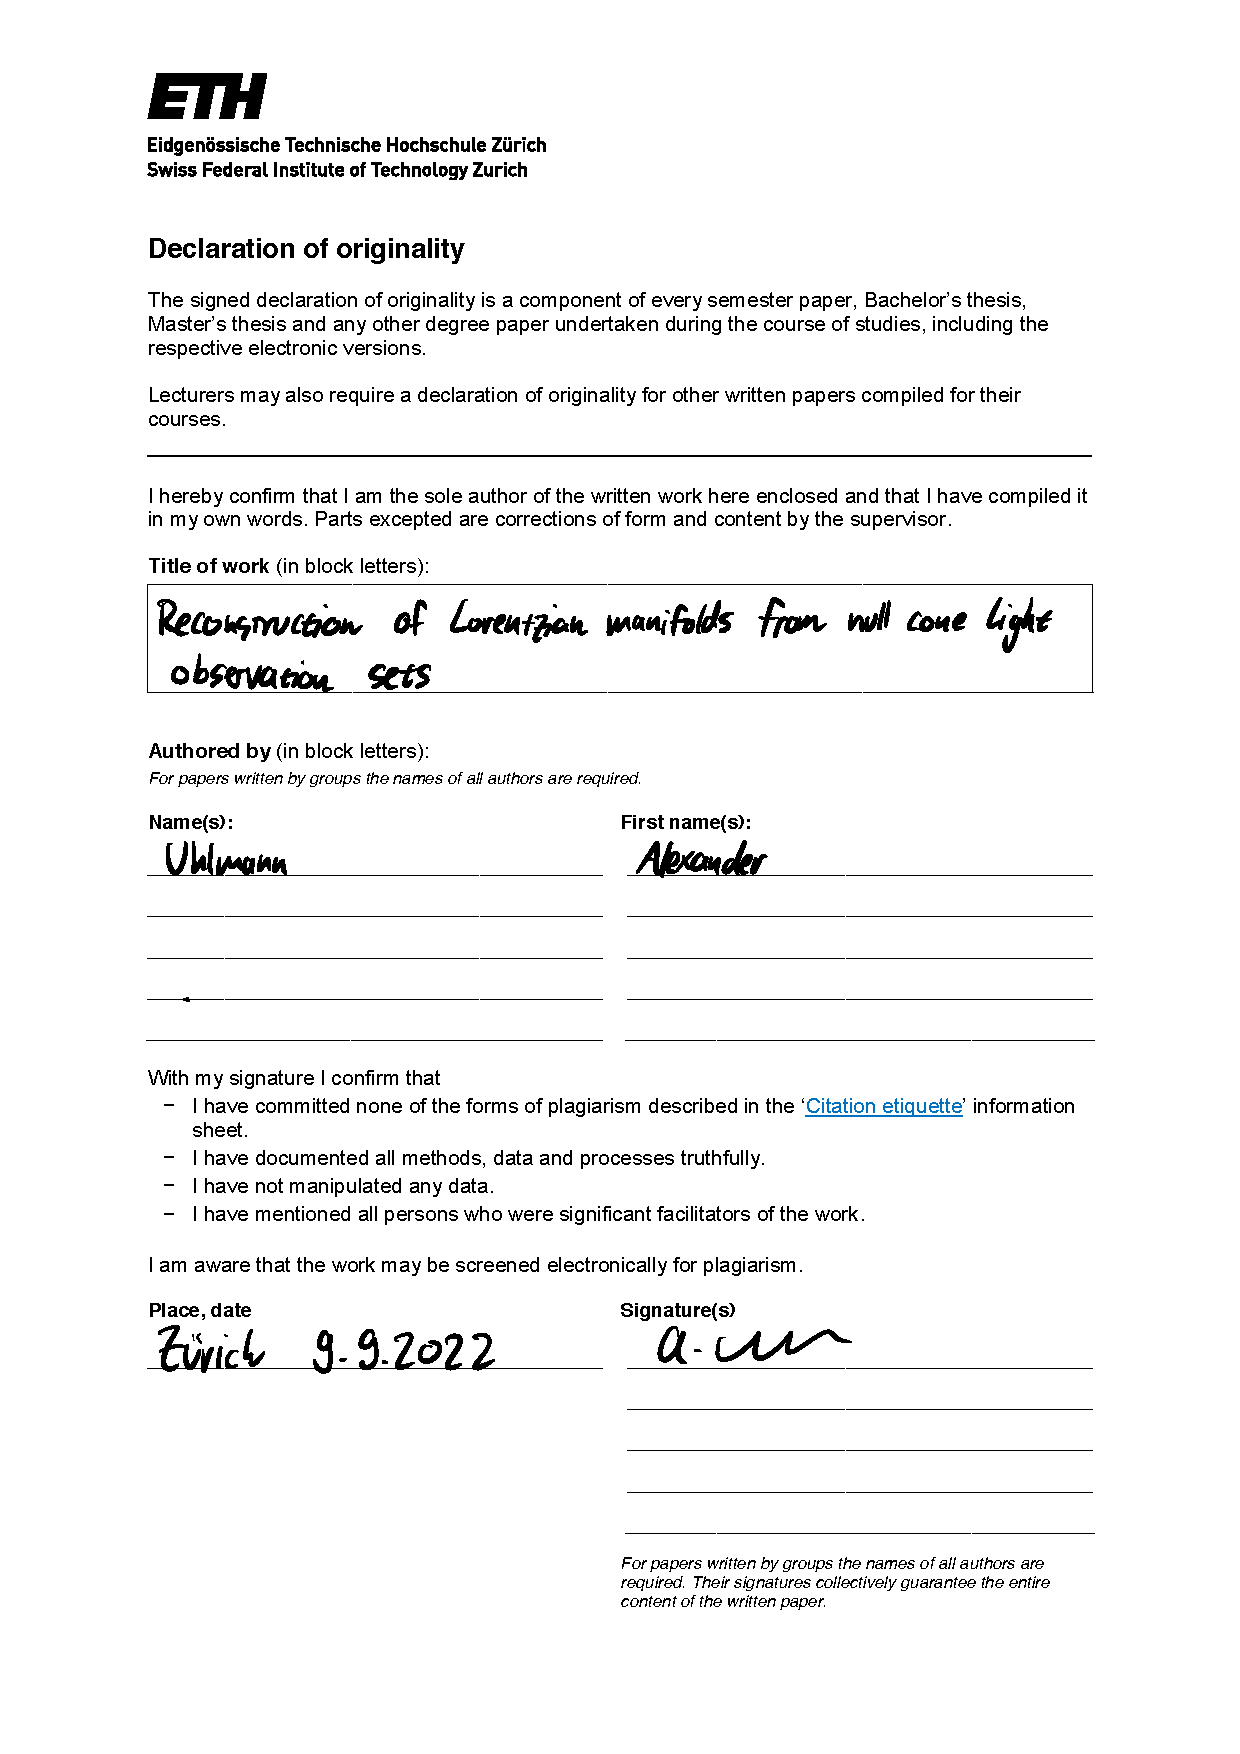
\includepdf[pages={-}]{declaration-originality.pdf}

\end{document}